\documentclass[extra, referee]{gji}
\usepackage{graphicx}

\usepackage{caption}

\usepackage{amsmath}
\usepackage{float}
\usepackage{multirow}

\usepackage{algorithm}
\usepackage{algorithmicx}
\usepackage{algpseudocode}
\usepackage{subcaption}

\usepackage{booktabs}

\newcommand{\norm}[1]{\left\lVert#1\right\rVert}

\renewcommand{\thefootnote}{\fnsymbol{footnote}}

\providecommand{\keywords}[1]{\textbf{\textit{Index terms---}} #1}

\begin{document}

\title{Research on 3D adaptive finite-element forward modeling and geometric multigrid preconditioner for direct current resistivity method}
\author[Ce Qin]{Ce Qin$^{1}$, WenLiang FU$^{1}$, Ning Zhao$^{1}$ \\
  $^{1}$Department of Physics and Electronic Information,
  Henan Polytechnic University, Jiaozuo, 454000, China
}

\maketitle

\begin{abstract}
In recent years, the Multigrid Method and Adaptive Finite Element Method have
been  applied to enhance the precision of numerical solutions in
three-dimensional direct current resistivity forward and inversion problems. The
hanging nodes caused by adaptive refinement, has enhance the computational
complexity of these simulations. To boost the efficiency of numerical
simulation, algebraic multigrid methods have been used as preconditioner in
Krylov space solvers in recent years. However, Algebraic Multigrid struggles
with poor convergence when handling high-order basis functions, leading to
significantly increased computational time.

Our study introduces a Conjugate Gradient method using geometric multigrid as a
preconditioner combine with the adaptive finite element method for
three-dimensional direct current resistivity forward simulations. This method
aims to enhance both solution accuracy and efficiency while mitigating
computational expenses. By leveraging a goal-oriented adaptive finite element
method based on posterior error estimators, our approach selectively refines
grids exhibiting substantial errors during the adaptive process.

The geometric multigrid method, based on geometrically partitioned grid
hierarchies, the smoothing at each level involves the current level and finer
levels only. When applied to adaptive grids, the degrees of freedom at each
level in the multigrid are low, lowering the data transfer costs between
adjacent levels, thereby enhancing the solution efficiency.

Our algorithm's effectiveness and parallel performance are confirmed through the
solution of the half-space model using both global and adaptive refinement
strategies. The outcomes confirmed our algorithm's ability to achieve more
accurate numerical solutions at significantly lower computational costs. Various
models, encompassing layered structures, complex terrain models constructed by
octree-based grid refinement methods, and unstructured grid models, are
subjected to simulations using geometric multigrid and Algebraic Multigrid
methods employing high-order basis functions. Schlumberger soundings to generate
pseudosection, validated geometric multigrid's capacity to deliver accurate
numerical solutions in solving complex models and comparative analysis of
convergence rates underscores the supremacy of geometric multigrid in resolving
three-dimensional direct current problems.

% Additionally, simulations employing geometric multigrid and algebraic
% multigrid on grids with distinct stretch factor demonstrate that geometric
% multigrid shows better solving efficiency and stability as the condition
% number of the linear system increases.

% Using the Message Passing Interface parallel protocol, numerical simulations
% of the half-space model are conducted under various processes to validate the
% parallel performance of geometric multigrid methods. Finally, we employ a
% model with complex topographies building with an octree-based grid refinement
% method and use Schlumberger soundings to generate pseudosection, validated
% geometric multigrid's capacity to deliver accurate numerical solutions in
% solving complex models.

\end{abstract}

\begin{keywords}
Direct current resistivity method, Geometric multigrid method, Adaptive finite
element method, Three-dimensional forward modeling
\end{keywords}

\section{Introduction}
The direct current (DC) resistivity  method is a widely recognized geophysical
exploration technique used to effectively detect conductive structures in the
shallow subsurface. It has extensive applications in various fields, including
mining exploration, civil engineering, hydrology, and environmental surveys.
Three-dimensional forward modeling is the basis of inversion and allows for the
design of observation systems based on forward the modeling results.
Three-dimensional forward modeling techniques can be classified into three
primary types based on the principles they employ: integral equation method
\citep{Hvodara1998,Mirgalikyzy2015,Huang2022,He2023}, finite difference method
(FDM) \citep{Spitzer1995,Wang2001,Edigbue2023,Yang2023}, and finite element
method (FEM)
\citep{Bibby1978,Li2005,Cai2017,Karaoulis2013,Johnson2017,Laksono2023,Hafsa2023}.
In particular, the finite element method offers several advantages when compared
to other methods. It provides higher solution accuracy and can relatively easily
handle complex geometric shapes, general boundary conditions, spatial
variations, and nonlinear material properties.

Solving linear equation systems is a critical component within the forward
modeling process. The solving process of the three-dimensional direct current
forward modeling often involves a large computational domain, leading to a large
number of unknowns in the forward equation systems. Direct solution methods are
impractical in such cases. Typically, iterative algorithms based on Krylov space
are employed for solving these equations, such as the conjugate gradient
\citep{Kronbichler2022,Guo2023,Amdouni2022} method used in this study. To
enhance the efficiency of the forward simulation, it is common to utilize
preconditioning techniques like successive over relaxation method \citep{Li2023}
and block Jacobi methods \citep{Haleem2023}. In recent years, to accelerate the
solving process, scholars have made significant progress . However, several
challenges still exist. For instance, there are issues related to high
computational complexity, significant computing time, and difficulties in
ensuring calculation accuracy.

Algebraic multigrid (AMG) is an efficient approach for solving linear equation
systems \citep{Okusanya2004,Farris1998,Wang2023}, it effectively addresses all
error components across low to high frequencies. AMG constructs the hierarchy
directly from the system matrix without the need for geometric information,
making it suitable as a black-box preconditioner for use with different
iterative schemes. However, it can not converge effectively when dealing with
high-order problems. In geophysical 3-D modeling, geometric multigrid
(GMG)\citep{Pan2022,Teunissen2023,Munch2023} is considered as the best approach
available to date. The GMG algorithm defines coarse and fine grids based on
geometric partitioning, while the interpolation and restriction operators
between different grid levels are determined by linear interpolation. The main
distinction between AMG and GMG lies in how they define the transfer operators
between coarse grids and grid levels. Compared to AMG, GMG requires less memory
and offers higher computational efficiency. GMG can be used both as a solver and
as a preconditioner for Krylov subspace \citep{Lu2014,HerreroPrez2023,Ilin2023}
methods to solve linear equation systems. Currently, multiple-grid algorithms
are actively studied in geophysics,  but there has been limited research on GMG
specifically for adaptive grids.

In this paper, we combined the adaptive finite element method  with GMG for
solving three-dimensional DC problems. We derived the control equations for 3-D
DC problems and conduct a finite element analysis. To obtain high-precision
solutions, it's necessary to refine the grid. However, conventional global
refinement results in large-scale problems, seriously affecting the efficiency
of solving differential equations. Therefore, we employ a goal-oriented adaptive
refinement method \citep{Ren2013,Wu2023,Becker2022} to selectively refine
regions with significant errors. This approach helps to avoid unnecessary global
mesh refinement due to the non-goal oriented approach or the use of prior
information to refine the grid. In order to enhance the convergence of solutions
and handle possible ill-conditioned matrices that may result from adaptive
refinement, we employ the block Jacobi \citep{Hoagland2021,Anzt2017,Yang2023a}
as the smoothing operator for GMG. Experimental results demonstrate that, GMG is
more suitable for solving three-dimensional DC electric problems and GMG
demonstrated good performance in solving adaptive grids.


% The direct current (DC) method is widely used in the fields of geophysical
% exploration and resource exploration in \citep{}. The finite element method
% \citep{Um2012,Vamaraju2020,Gassmller2019}, known for its broad adaptability,
% high accuracy, strong reliability, and good scalability, is a numerical method
% commonly employed in geophysical exploration. In recent years, scholars have
% made significant progress with material property modeling in
% \citep{Bergamo2014}, algorithm optimization in \citep{Schwarzbach2005},
% parallel computing in \citep{Feng2021} and deep learning in
% \citep{Puzyrev2019}. However, several challenges still exist. For instance,
% there are issues related to high computational complexity, significant
% computing time costs, and difficulties in ensuring calculation accuracy. This
% approach helps avoid unnecessary global grid refinement caused by
% non-goal-oriented approach or artificial grid refinement using prior
% information.

% Firstly, there is the issue of high computational complexity. Solving
% large-scale linear equation systems with the finite element method results in
% a high computational complexity. In some cases, the convergence time is
% excessively long or achieving convergence precision becomes impossible.
% Secondly, a significant computational time is incurred. For 3-D problems, a
% substantial number of nodes need to be calculated, leading to extensive
% calculations that require a long computation time and massive storage space.
% Thirdly, calculation accuracy poses a challenge. The DC 3-D finite element
% method requires grid partitioning during the discretization of space. However,
% different grid partitioning methods and selected basis functions can impact
% the numerical solution, resulting in increased numerical errors.

% In previous studies, three-dimensional forward modeling predominantly employed
% algebraic multigrid (AMG) method, for instance, in
% \citep{Codd2017,Koldan2014}, however, its solving speed is not remarkable when
% solving large-scale linear systems. In order to further address the issue of
% high computational complexity and convergence difficulties, we used geometric
% multigrid (GMG) technique \citep{Pan2022,Teunissen2023}. In order to handle
% possible ill-conditioned matrices that may result from adaptive refinement, we
% have chosen the block Jacobi method as the smoother operator
% \citep{Hoagland2021,Anzt2017}. Experimental results demonstrate that, compared
% to the Algebraic Multigrid (AMG) method, GMG exhibits faster convergence rates
% and requires fewer convergence steps in various grid environments. These
% results indicate that GMG is more suitable for solving three-dimensional DC
% electric problems.

% In this paper, we apply a parallel algorithm based on the MPI protocol
% \citep{Patel2022,Izaguirre2005} to further accelerate the solving speed and
% investigate the scalability of adaptive algorithms. With the exception of
% model building, all steps involved in solving the equation, including matrix
% assembly, matrix solving, and posterior error estimation, can be parallelized.
% The speedup serves as an essential indicator of parallel computing
% performance. We demonstrate that the GMG algorithm exhibits good scalability
% by studying the performances in the speedup for different grid environments.
% In the example where the number of degrees of freedom is 14 million, the
% adaptive algorithm still demonstrates excellent scalability, indicating the
% applicability of the GMG method to large-scale parallel computing.

% To validate the feasibility of the GMG method in complex model environment, we
% conducted forward modeling on a grid containing multiple anomalous bodies.We
% established grids by using the octree technique \citep{Teunissen2023}
% andextracted potential information from the forward modeling. By combing the
% forward modeling results with the geometric information of the observation
% device, we utilized the Schlumberger sounding to generate a pseudo-section
% plot \citep{Ogunbo2018}. The results show that the GMG method is capable of
% effectively acquiring potential information with high accuracy, even in
% complex subsurface structures.

\section{DC 3-D Adaptive Finite Element Method}
\subsection{Boundary value problem and weak form}
In a steady current field, the electric field $\mathbf{E}$, current density
$\mathbf{J}$, and potential $u$ obey the differential form of Ohm's Law in
physics \citep{Kaufman2014,Kovaevi2022}. The relationship between them is as
follows:
\begin{equation}
  \label{eq:Ohm}
  \mathbf{J}=\sigma \mathbf{E}.
\end{equation}

Here $\sigma$ represents conductivity, and $\mathbf{E}$ satisfies:
\begin{equation}
  \label{eq:EV}
  \mathbf{E}=-\nabla u.
\end{equation}

We place a point source on the ground surface $\Gamma_s$, the current is I.
According o the law of conservation of charge \citep{Horndeski1976,OConnor2022},
the continuity equation of the current can be obtained as follows:
\begin{equation}
  \label{eq:charge}
  \nabla \cdot \mathbf{J}=I \delta( \mathbf{A}),
\end{equation}
where $\delta(\mathbf{A})$ is the Dirac Functions. Substituting equations
\ref{eq:Ohm} and \ref{eq:EV} into equation \ref{eq:charge}, the differential
equation that the potential must satisfy can be obtained as follows:
\begin{equation}
  \label{eq:fist}
  \nabla \cdot (\sigma\nabla u ) = -2 I \delta( \mathbf{A}) \in \Omega,
\end{equation}
where $\mathbf{A}$ is the field source point position which located on the
surface $\Gamma_s$, $ \Omega$ represents the entire computational domain. On the
surface $\Gamma_s$, the normal derivative of the potential satisfies
\begin{equation}
  \label{eq:second}
  \frac{\partial{u}}{\partial{n}}=0 \in \Gamma_s.
\end{equation}

We define the infinite boundary as $\Gamma_\infty$, the potential here is
linearly related to the distance from point $\mathbf{A}$, and the distribution
of the potential satisfies
\begin{equation}
  \label{eq:third}
  u=\frac{c}{r}\in \Gamma_\infty,
\end{equation}
where $c$ is a constant, $r$ is the distance from point $\mathbf{A}$. By taking
the derivative of the above equation and eliminating the constant, the following
equation can be obtained:
\begin{equation}
  \label{eq:forth}
  \frac{\partial{u}}{\partial{n}}+\frac{cos(\mathbf{r}, \mathbf{n})}{r}u=0\in \Gamma_\infty.
\end{equation}

The above equations \ref{eq:fist} to \ref{eq:forth} constitute a
three-dimensional electric field boundary value problem, and the resistivity
interface inside the region $\Omega$ serving as the natural boundary value
condition.
\begin{figure}
  \centering
  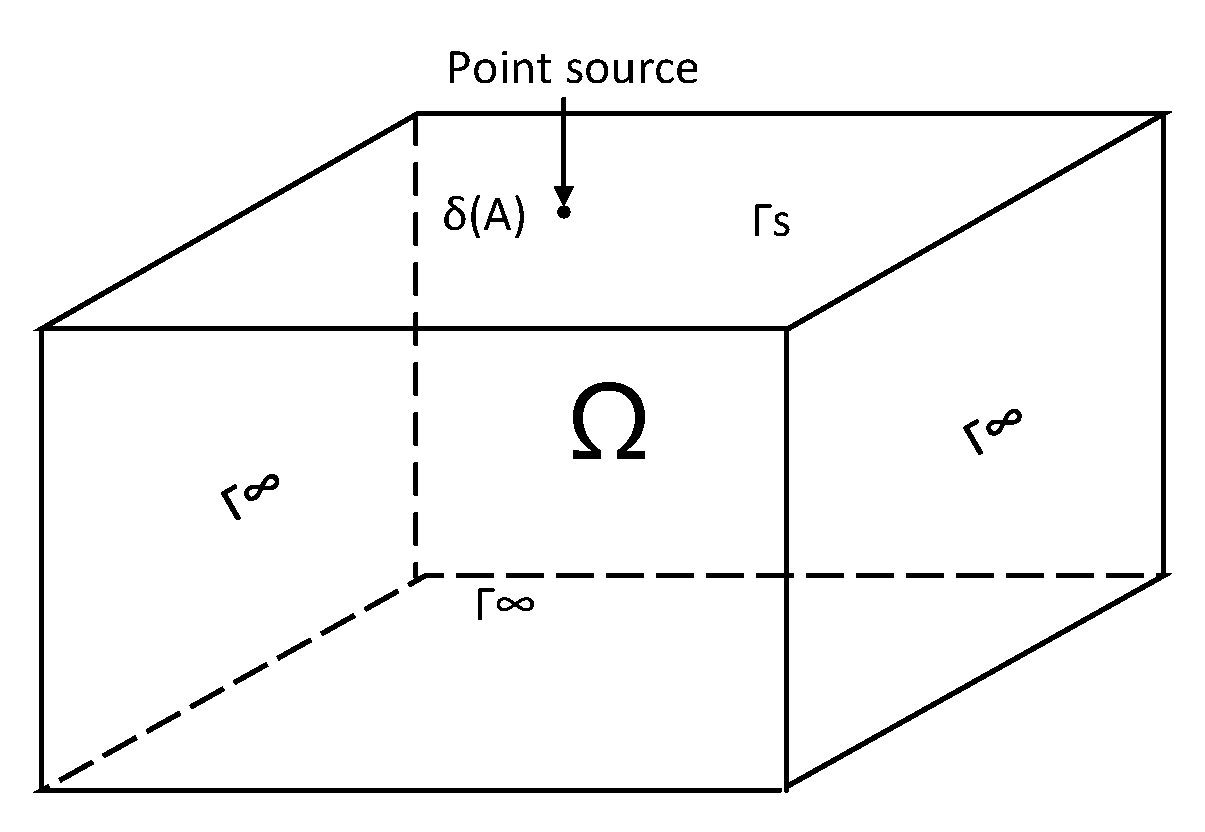
\includegraphics[width=0.6\textwidth ]{fig/compute_domain.pdf}
  \caption{Schematic diagram of calculation domain, $ \Omega$ represents the entire computational domain and $\Gamma_\infty$ is the infinite boundary. $\Gamma_s$ is the horizontal ground surface and a point source $\delta(\mathbf{A})$ is located on the $\Gamma_s$ }
  \label{fig:compute_domain}
\end{figure}

We multiply the test function $\phi$ by both sides of equation \ref{eq:fist} and
integrate, resulting in:
\begin{equation}
   \label{eq:testfun}
   \int_{\Omega} \phi\nabla \cdot(\sigma\nabla u )= \int_{\Omega} -\phi 2 I \delta( \mathbf{A}).
\end{equation}

In order to obtain the weak form of the differential equation, we perform
integral by parts on the left-hand side of equation \ref{eq:testfun} and apply
Gauss's theorem. Substituting equation \ref{eq:forth} into the above equation,
the following result is obtained:
\begin{equation}
  \label{eq:testfun1}
  \int_{\Omega} \nabla \phi \cdot (\sigma \nabla u) {d}\Omega + \int_{ \Gamma_\infty}\phi\frac{ {cos}(\mathbf{r}, \mathbf{n})}{r} {u} {d}\Gamma= \int_{\Omega}\phi 2 {I} \delta( \mathbf{A}) {d}\Omega.
\end{equation}

In order for the test function $\phi$ to satisfy all boundary conditions, the
weak form should be expressed as follows:
\begin{equation}
  \label{eq:testfun2}
  (\nabla \phi, \sigma\nabla u )+ (\phi, \frac{ {cos}(\mathbf{r}, \mathbf{n})}{r} u)_{\Gamma_s}= (\phi, 2 I \delta( \mathbf{A})).
\end{equation}

The discrete representation of the weak form has the following form:
\begin{equation}
  \label{eq:testfun3}
  (\nabla {\phi_i}, \nabla u_ h)=\left(\nabla\phi_i, \nabla \left[\sum_{j} U_ {j}\phi_\mathbf{j} \right]\right)=\sum_ {j}(\nabla\phi_ {i}, \nabla\phi_ {j}) {U}_{j}.
\end{equation}

Set $\mathbf{A}_{ij}=(\nabla\phi_i, \nabla\phi_j)$, $\mathbf{b}_i=(\phi_i, 2 I
\delta( \mathbf{A}))$, this transforms the problem into finding a vector
$\mathbf{x}$ that satisfies $\mathbf{A}\mathbf{x}=\mathbf{b}$ in the selected
discrete domain. The equation \ref{eq:testfun3} is called primal problem.

To solve equation \ref{eq:testfun2}, we develop a three-dimensional model and
divide the  computational domain into numerous elements. For a 3-D problem, it
is necessary to compute a lot of nodes, leading to a very high computational
complexity and significant time expenditure during the solving process.
% In order to solve equation , we establish a model in three-dimensional space
% and discretize it to divide the computational domain into multiple elements.
% For a three-dimensional problem, a large number of nodes need to be computed,
% and the resulting computational complexity poses significant time and memory
% costs when solving the linear system.
When faced with high computational complexity, the stability of solvers often
deteriorates, leading to a significant increase in the solving time. In some
cases, the solver may even fail to converge due to the inability to attain the
desired convergence accuracy or encountering memory limitations.

The main idea of this paper is to enhance solving efficiency through two key
strategies: reducing the problem size and implementing efficient solution
methods. The adaptive finite element method is employed to reduce degree of
freedom while maintaining the accuracy of the grid solution. The GMG method is
regarded as an effective and stable approach for solving partial differential
equations, and it will be applied to solve complex partial differential equation
systems in this paper.


\subsection{ Adaptive finite element method}
% In order to improve the accuracy of the solution at points of interest, grid
% refinement becomes imperative when tackling the DC 3-D problem through the
% finite element method.
To enhance solution accuracy at critical points, grid refinement is essential
when dealing with the DC 3-D problem using the finite element method. Global
refinement can improve precision but comes at the cost of a substantial increase
in degrees of freedom, leading to a severe reduction in computational
efficiency. To optimize both solution accuracy and computational efficiency, we
adopted the adaptive finite element method. This strategy selectively enhances
grid density in specific regions, facilitating a more efficient allocation of
computational resources.

The posterior error estimator \citep{Mu2019,Ren2013,Ray2023,Wen2023} is a
crucial technique for determining which cells need further refinement in this
study. The posterior error is determined by assessing the numerical solution's
error on the current grid. Subsequently, only cells exhibiting substantial
errors undergo additional refinement. This selective refinement process helps
concentrate computational efforts where they are most needed, contributing to an
improved overall solution accuracy.

Considering the physical behavior of electric fields, it is imperative for the
current density within hexahedral elements to adhere to the continuity
constraint on internal surfaces. However, ensuring continuity of the normal
component of the total current density $\mathbf{J}$ within the $\Omega$ space
presents challenges. Assessing the consistency of conditions associated with
electric field continuity serves as a method to estimate the numerical errors of
finite element. The evaluation method can be employed to guide the adaptive
refinement process of the grid, thereby enhancing the local accuracy of the
solution. For the hexahedral element $e$, based on the principles mentioned
above, we can formulate the following expression for the posterior error
estimator:
\begin{equation}
  \label{eq:estimate}
  [\eta^{r}_{e}]^2 =\frac{1}{2} h_F [{\mathbf{n}} \cdot \mathbf{J}]^2_F.
\end{equation}

We define $f$ as the set of six quadrilaterals that constitute the
hexahedral element $e$, $h_f$ represents the maximum diameter of the
quadrilaterals in $f$,$\mathbf{n}$ is the normal vector of the shared
face of two hexahedral elements. The factor of 1/2 arises from the jump across
the shared face of two hexahedral elements. Equation \ref{eq:estimate} signifies
the contribution arising from erroneous surface charges that accumulate due to
discontinuous surface currents.

To adaptively refine the grid within the region of interest, we introduce a dual
problem. In this context, we create an additional right-hand term, denoted as
$\mathbf{b}_{d}$, by introducing a point source $\delta(\mathbf{N})$ at each
observation point position, where $\mathbf{N}$ represents the position of
observation point. We then solve for $\mathbf{x}_{d}$ by addressing the equation
$\mathbf{A}\mathbf{x}=\mathbf{b}_{d}$ within the same computational domain as
the primal problem.

By evaluating the posterior error of both $\mathbf{x}$ and $\mathbf{x}_{d}$, it
becomes possible to determine the posterior error for both the primal problem
and its dual problem. After weighting the errors between the two, grid
refinement can be executed on cells exhibiting larger errors. This
implementation of selectively refining within regions of interest is commonly
known as goal-oriented adaptive refinement. In the following discussion, we will
provide a brief overview of the operational details of this method.

We define the self-adjoint symmetric bilinear form $B(, )$ as follows:
\begin{equation}
  \label{eq:testfundual0}
   B(\mathbf{E}, \mathbf{V}) = \int_{\Omega} \nabla \mathbf{V} \cdot (\sigma \nabla \mathbf{E}) {d}\Omega + \int_{ \Gamma_\infty}\mathbf{V}\frac{ {cos}(\mathbf{r}, \mathbf{n})}{r} {\mathbf{E}} {d}\Gamma,
\end{equation}
where $\mathbf{V}$ is a vector test function.

We define the linear function of the potential as $L(\mathbf{M})$, where
$\mathbf{M}$ is the accurate solution of the electric field and belongs to
$\Omega$  \citep{Ren2013}. The adaptive algorithm aims to minimize errors within
the specified area of interest. The  primary weak form of its corresponding
primal problem is derived as follows:
\begin{equation}
  \label{eq:testfundual11}
   B(\mathbf{E}, \mathbf{V}) = L(\mathbf{V}).
\end{equation}

Then the primary weak form of the dual problem can be defined, which seeks to
find $\mathbf{U} \in \Omega$, such that
\begin{equation}
  \label{eq:dualweak}
   B(\mathbf{U}, \mathbf{V}) = L(\mathbf{V}).
\end{equation}

In the dual weak form of equation \ref{eq:dualweak}, $L(\mathbf{V})$ is a linear
functional acting on an arbitrary function $\mathbf{V}$ within the domain
$\Omega$. The solution $\mathbf{U}$ to the dual problem is commonly known as the
'influence function' \citep{Oden2001}. Additionally, we define the numerical
error of the potential as $\mathbf{e} = \mathbf{M} -\mathbf{M}_h$, where
$\mathbf{M}_h$ signifies the numerical solution of primal problem. With these
definitions, we obtain the following formula:
\begin{equation}
  \label{eq:testfundual1}
   L(\mathbf{e})=B(\mathbf{U}, \mathbf{e}) = B(\mathbf{U}_h, \mathbf{e})
     + B(\mathbf{u}_e, \mathbf{e})=B(\mathbf{u}_e, \mathbf{e}).
\end{equation}

The error value of $\mathbf{U}$ is denoted as $\mathbf{u}_e$, and $\mathbf{U}_h$
represents the finite element approximation of $\mathbf{U}$. Due to the Galerkin
orthogonality property in \citep{Brenner2008}, we have $ B(\mathbf{U}_h,
\mathbf{e}) = 0$. To explicitly express $B(\mathbf{u}_e, \mathbf{e})$, we apply
the Cauchy-Schwartz \citep{Oden2001,Brenner2008} inequality on equation
\ref{eq:testfun1}:
\begin{equation}
  \label{eq:testfundual2}
   \left| L(\mathbf{e}) \right| = \left| B(\mathbf{e}, \mathbf{u}_e) \right|
     \leq \sum_{n=1}^{N} \left| B_n(\mathbf{e}, \mathbf{u}_e) \right|
     \leq \sum_{n=1}^{N} ||\mathbf{e}||_{e, n} \ ||\mathbf{u}_e||_{e, n}
     \approx \sum_{n=1}^{N} C_n \ ||\mathbf{e}||_{L^2, n} \ ||\mathbf{u}_e||_{L^2, n}.
\end{equation}

In the given equation, $C_n$ is a positive constant influenced by cell size,
impedance, and conductivity. The norm $||.||_e$ represents the energy norm of
the bilinear form$ B(,)$, defined as $||.||_e = \sqrt{|B(,)|}$. The L2 norm
\citep{Zdunek2005} serves as a substitute for the energy norm. This substitution
alleviates computational challenges associated with assessing errors in the
energy norm while preserving the efficiency of error estimation. We redefine the
following parameters: $\eta_d = ||e||_{L^2,n}$ as the error indicator for
$\mathbf{M}$, $\eta_d = ||\mathbf{u}||_{L^2,n}$ as the error indicator for
$\mathbf{U}$. Then, the error estimator for $L(\mathbf{e})$ is given by:
\begin{equation}
  \label{eq:testfundual3}
   \eta = \sum_{n=1}^{N} \eta_p \cdot \eta_d.
\end{equation}

As indicated in Equation \ref{eq:testfundual3}, the error indicator for
goal-oriented adaptive refinement is determined by the product of the error
estimates for both the primal and dual problems. By employing this resulting
error estimator, denoted as $\eta$, it becomes feasible to exclusively perform
refinements within the regions of interest. This achieves the objective of
enhancing both accuracy and computational efficiency simultaneously.

\section{ Geometric Multigrid Method}
% The GMG method possesses several advantages, including efficient solving
% speed, high precision in solution accuracy, adaptability, and parallel
% scalability. These features make it a vital tool for dealing with large-scale
% scientific computing problems. Previous research mainly focused on uniform
% grids. However, in this study, we aim to improve the solving speed further by
% employing the GMG method on adaptively refined grids. In fine-grained grids,
% low-frequency errors are difficult to eliminate, leading to slow convergence
% in iterative solvers. Geometric multigrid (GMG) methods utilize the
% relationships between different levels to effectively eliminate low-frequency
% errors. Thus, we will apply the GMG method on the adaptively refined grid to
% significantly improve the solution speed.

%  The GMG method hierarchy is applicable for handling problems with complex
% geometric shapes, as it can capture different scale features at different grid
% levels. In the iterative process, each linear equation system that needs to be
% solved requires a preconditioner to provide an initial solution vector and a
% preconditioning matrix. The purpose of the preconditioner is to enhance the
% convergence of the iterative process and decrease the computational cost.
% Solving the three-dimensional direct current problem will encounter huge
% problem sizes, large-scale parallel computing methods will be considered to
% accelerate the solution process. Geometric multigrid has demonstrated
% excellent performance in large-scale parallel computing over the past four
% decades.

\subsection{V-cycle}

For the given L-level grid structure, we introduce the concept of active cells
within the hierarchical structure ${\mathbf{T}_l}$ $(0 \leq l \leq L)$. For the
grid $\mathbf{T}_l$, finite element basis functions are introduced, and a linear
system of equations is constructed to compute the approximate solution of
$\mathbf{b}$ on the current grid. Linear system on $\mathbf{T}_l$ can be
represented as $ \mathbf{A}_l \mathbf{x}_l = \mathbf{b}_l$.

To solve this system, the conjugate gradient (CG) method
\citep{Lotfi2020,Yousif2022} is employed. In the CG method, a new iteration is
created using the residual $\mathbf{r}_k$ from the current iteration step k.
Although these methods employ orthogonalization techniques to minimize the next
iteration and enhance performance \citep{CheikAhamed2012}, their computational
speed experiences a noticeable decrease when applied to fine grids. The
following formula demonstrates a part of the conjugate gradient method:
\begin{equation}
  \label{eq:CGpart}
   \mathbf{r}^{k+1}_l=\mathbf{r}^{k}_l+\omega \mathbf{r}^{k}_l,
\end{equation}
where $ \mathbf{r}{_l}^{k} = \mathbf{A}_l \mathbf{e}_{l}^k = \mathbf{b}_l -
\mathbf{A}_l \mathbf{x}{_l}^k$ represents the residual of step k, while
$\mathbf{e}^k = \mathbf{x} - \mathbf{x}^k$ denotes the error between the true
solution and the iterative solution at step k.

We used multigrid method to overcome the issues above. To expedite convergence,
a preconditioner is introduced, mapping the residual back to a function
\citep{Janssen2011}. We define the preconditioner of the geometric multigrid as
$\mathbf{P}$ , the smoothing operator as $\mathbf{S}_l^{(i)}$ and the
restriction operator as $\mathbf{R}{_l}^{T}: \mathbf{V}_l \rightarrow
\mathbf{V}_{l+1}$. To introduce the classic V-cycle algorithm, we define: $m_l$
as the number of iterations for pre-smoothing, and the number of iterations for
post-smoothing is the same as for pre-smoothing. In the coarse grid correction
phase, only one iteration is involved. Then the action of $\mathbf{P}_l^{-1}$ on
the residual vector $\mathbf{d}_l$ can be recursively expressed using the
following algorithm:
\begin{algorithm}  %生成浮动式图
    \caption{V-cycle.}  %标题
    % 由algorighmic完成代码的编译部分
    \label{eq:algorithm1}

    \begin{algorithmic}[1] %[1]表示每行显示行号, 且由123.. 排序
        \State Let $\mathbf{P}_0 = \mathbf{A}_0$ and $\mathbf{x}^{(0)} = 0$.
        Then, the action of the operator $\mathbf{P}_l^{-1}$ on a vector
        $\mathbf{d}_l$ is defined as follows: \State Pre-smoothing: Compute
        $\mathbf{x}^{(m_l)}$ iteratively by

        $\mathbf{x}^{(i)} = \mathbf{x}^{(i-1)} + \mathbf{S}^{(i)}
        _l(\mathbf{d}^{(i)}_l - \mathbf{A}^{(i)}_l \mathbf{x}^{(i-1)}), \quad i
        = 1, \ldots, m_l.$


         \State Coarse grid correction: Let

        $ \mathbf{y}^{(0)} = \mathbf{x}^{(m_t)} + \mathbf{R}^{T}_{l-1}
        \mathbf{P}^{-1}_{l-1} \mathbf{R}_{l-1} \left( \mathbf{d}_l -
        \mathbf{A}_l \mathbf{x}^{(m_l)} \right). $ \State Post-smoothing:
        Compute $\mathbf{y}^{(m_l)}$ iteratively by

        $\mathbf{y}^{(i)} = \mathbf{y}^{(i-1)} + \mathbf{S}^{(m_l+i)}_l \left(
        \mathbf{d}_l - \mathbf{A}_l \mathbf{y}^{(i-1)} \right), \quad i = 1,
        \ldots, m_l.$ \State Set $\mathbf{P}^{-1}_l \mathbf{d}_l =
        \mathbf{y}^{(m_l)}.$

    \end{algorithmic}
\end{algorithm}

Algorithm \ref{eq:algorithm1} reports the iterative mode employed within the
geometric multigrid method. This algorithm begins by conducting a few iterations
on a finer grid to eliminate high-frequency errors. Subsequently, confine
low-frequency errors to a coarser grid. On the coarser grid, the low-frequency
errors from the finer grid morph into high-frequency components, allowing for
their effective elimination through a few times iterations. Continue this
process until you reach the coarsest grid, where the number of unknowns is
typically minimal, allowing for a direct, rapid, and precise solution. Finally,
interpolate the solution from the coarsest grid to the finer grids to rectify
the solutions on the finer grids. During each interpolation step, several
smoothing iterations are necessary to eliminate high-frequency errors introduced
by the interpolation process, continuing until you reach the finest grid.

As a form of nested iteration technique  \citep{SungLim2000}, the V-cycle
\citep{Chen2019,Ha2021} used in this paper efficiently converges to an accurate
solution when the number of levels in the multigrid is small. Fig.
\ref{fig:Vcycle} visually illustrates the processes of the the V-cycle.
\begin{figure}
  \centering
  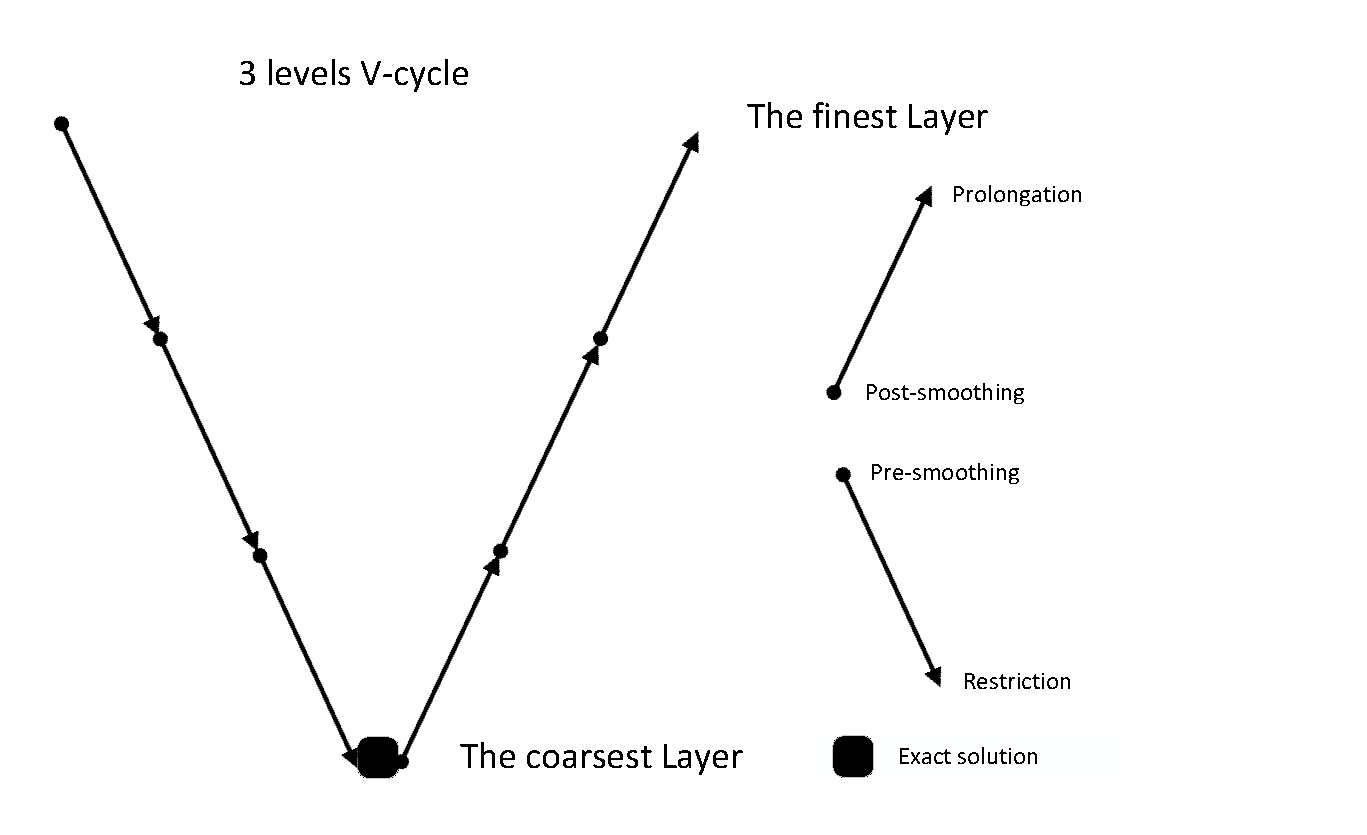
\includegraphics[width=0.8\textwidth]{fig/Vcycle.pdf}
  \caption{A schematic diagram of a three-level V-cycle, starting from the
    finest grid, undergoes three iterations to the coarsest grid, and then goes
    through three iterations back to the finest grid. The direction of the
    arrows indicates the direction of grid switching: downward signifies a
    switch to a coarser grid, while upward signifies a switch to a finer grid.
    The arrow's starting point represents either pre-smoothing or post-smoothing
    operations. The arrow's endpoint indicates the operation of transferring
    data from the current grid to a coarser or finer grid through restriction
    and prolongation operators.}
  \label{fig:Vcycle}
\end{figure}
The geometric multigrid method employs both the interpolation and restriction
operators, working collaboratively to transfer data across various levels. In
the iteration process of geometric multigrid, there is a need for transferring
data from coarse grids to fine grids. This transfer is typically accomplished
through interpolation operators. The interpolation method we used is
accomplished through linear interpolation techniques. On the other hand, the
restriction operator restricts high-precision grid data to low-precision grid.
As we approach finer grid, the data of high-precision grid is restricted  onto
lower precision grid by using weighted averaging methods to ensure the overall
convergence of the geometric multigrid method.

\subsection{ Splitting of grid into levels}
The Geometric Multigrid method splits the grid into various levels through local
smoothing and global coarsening coarsening. Implementing global coarsening is
uncomplicated, as all levels cover the entire computational domain, requiring no
consideration for internal interfaces. Data transfer between different levels is
achieved through simple copying operations from the finest level. At each
coarsening level, four adjacent nodes merge into a new node, typically
positioned as the average of neighboring nodes.
% Fig. \ref{fig:global} provides a visual representation of this coarsening
% process. \begin{figure} \centering 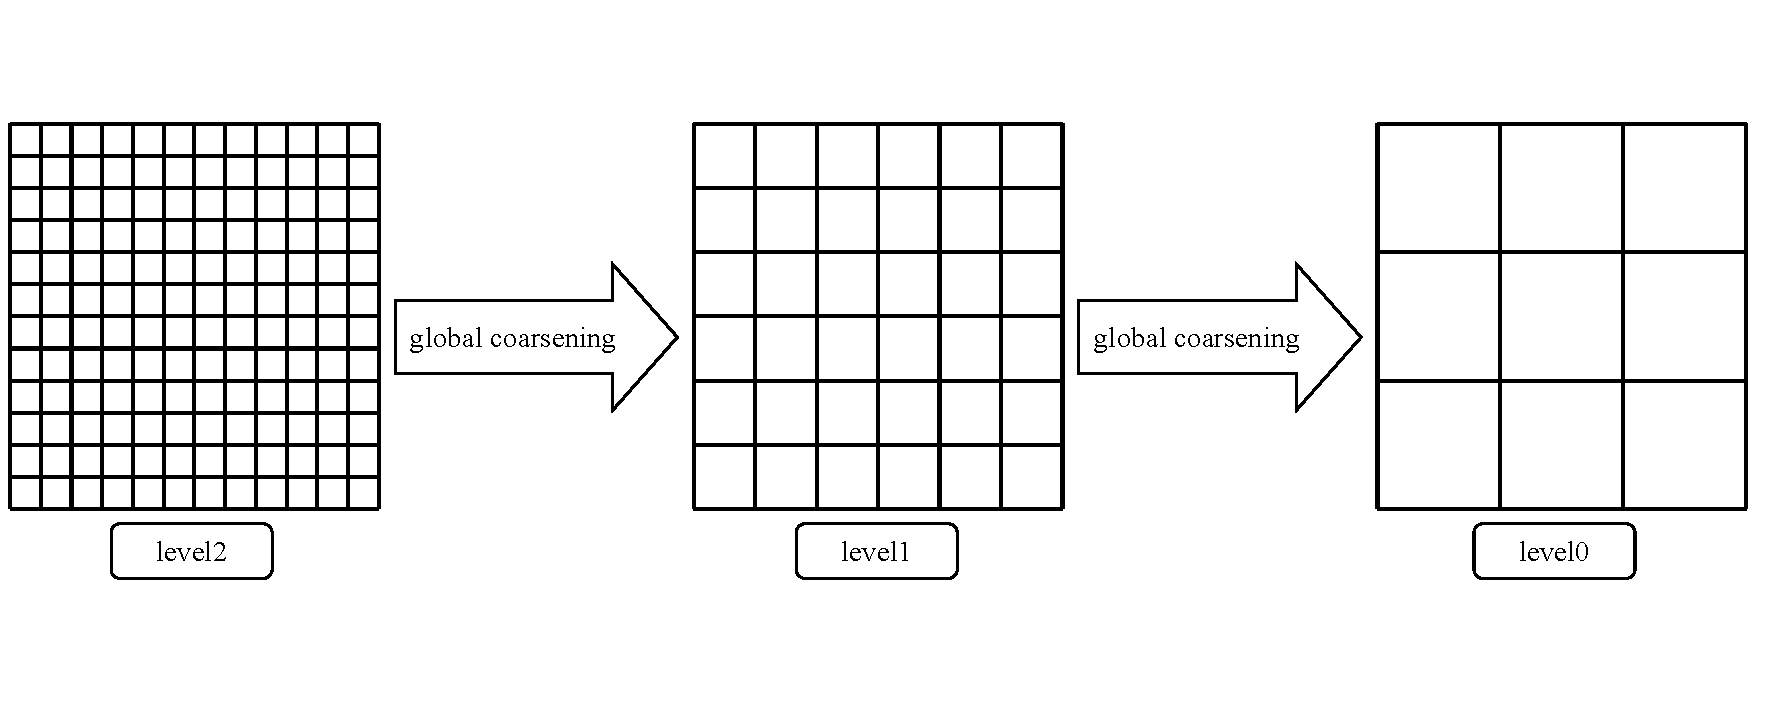
\includegraphics[width=1 \textwidth
% ]{fig/global.pdf} \caption{Splitting of uniform  grid into levels.}
% \label{fig:global} \end{figure}
\begin{figure}
  \centering
  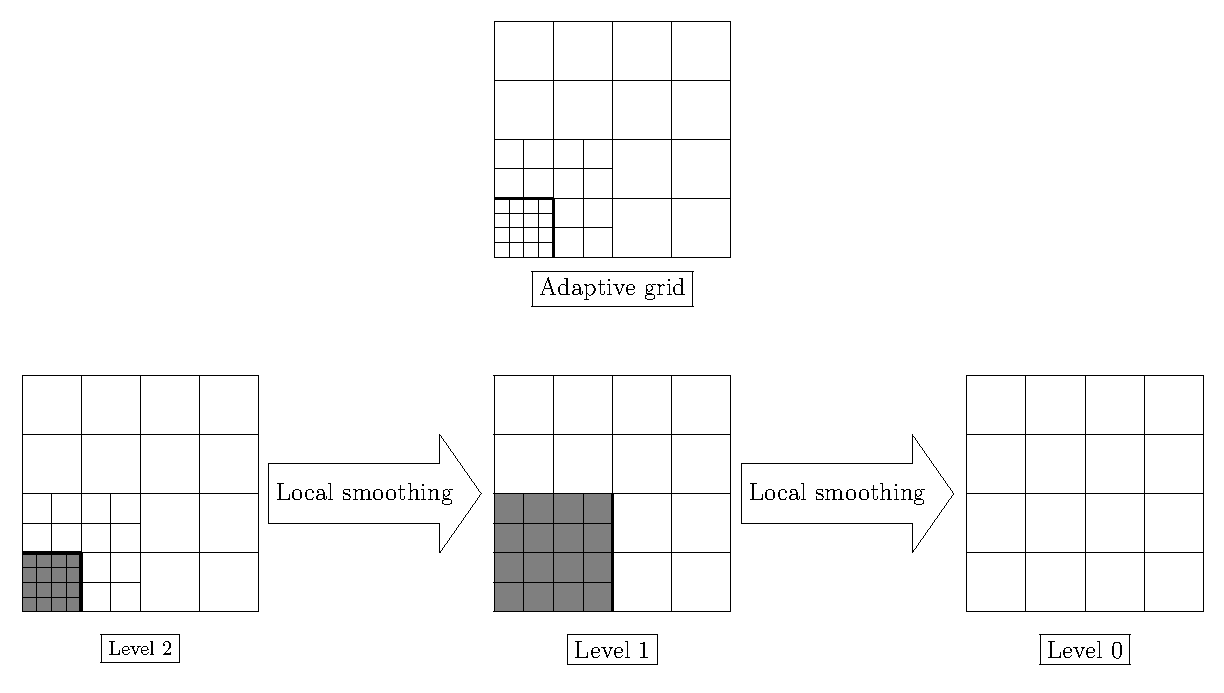
\includegraphics[width=1 \textwidth]{fig/local_smoothing.pdf}
  \caption{Splitting of adaptive grid into 3 levels through local smoothing. In
    the grids of level 2 and level 1, only the gray portion constitutes the grid
    level of this level. The entire grid of level 0 is considered as one grid
    level.}
  \label{fig:local_smoothing}
\end{figure}

In contrast to global refinement, adaptive refinement leads to substantial
variations in grid resolution in specific areas. As discussed in
\citep{Munch2023}, global coarsening leads to a certain number of hanging nodes
in the multigrid hierarchy. These hanging nodes disrupts the continuity of the
numerical solution and increases difficulty in solving the equations system.
Therefore, for adaptive grids, local smoothing is considered to split the grid
into levels.

After generating the grid through adaptive refinement, various pixel areas are
formed. The GMG method splits grids into levels through local smoothing
\citep{Munch2023,Bastian2006,Clevenger2021}. We describe the primary process as
follows: If there are cells of different sizes from the minimum size, all cells
with the smallest size within the grid are added into a collection which is
designated as a level of the multigrid hierarchy. The shaded area in Fig.
\ref{fig:local_smoothing} shows the collection of the smallest cells from adaptive grid,
which forms the finest level 2. The regions corresponding to these collected
cells undergo local smoothing to update the grid. These operations are repeated
iteratively if there are cells in the current grid that are different from the
minimum size, until all grid cells reach uniform size. Once all cells within the
current grid have achieved the same size, the entire grid can be considered as
the coarsest level 0.

As a result, smoothing at a specific level only involves the cells at the
current level and finer levels. Compared to global coarsening discussed in
\citep{Huang2023}, each level obtained using local smoothing algorithms has
lower degrees of freedom, reducing the cost of transfer between adjacent levels.
It is evident that as the refinement level increases, the adaptive grids benefit
from this specialized hierarchical approach that can provide more levels when
utilizing the same memory resources. When computational resources are limited,
this allows the geometric multigrid algorithm achieve higher precision solutions
and improve computational speed by utilizing deeper levels of grid hierarchy.

\subsection{Splitting of level spaces}

In the process illustrated in Fig. \ref{fig:local_smoothing},  cells of the same size are
grouped together as a level in the multigrid approach. This approach allows that
the horizontal matrices of the multigrid method can be easily assembled by
traversing all cells at a certain level, and these horizontal matrices do not
include hanging nodes.

Focus on the bolded part in level l of Fig. \ref{fig:local_smoothing}, we call the
degrees of freedom in this as edge degrees of freedom $(\mathbf{x}^E_l)$, while
the unknowns in the remaining part are called interior degrees of freedom
$(\mathbf{x}^S_l)$. Thus, the solution $\mathbf{x}_l$ to the differential
equation defined on level l can be expressed as $\mathbf{x}_l = \mathbf{x}^E_l +
\mathbf{x}^S_l$. Although these matrices are small, we still need to assemble
them and provide the necessary information to the multigrid method. In the
equation $\mathbf{A}_l \mathbf{x}_l =\mathbf{b}_l$, due to the decomposition of
$\mathbf{x}$, matrix $\mathbf{A}$ is also decomposed into $\mathbf{A}^{SS}_l$,
$\mathbf{A}^{ES}_l$, $\mathbf{A}^{EE}_l$, and $\mathbf{A}^{SE}_l$. Consequently,
the following equations can be derived:
\begin{equation}
  \label{eq:nine}
  \begin{pmatrix}
    \mathbf{A}^{SS}_l & \mathbf{A}^{SE}_l\\
    \mathbf{A}^{ES}_l & \mathbf{A}^{EE}_l\\
  \end{pmatrix}
  \begin{pmatrix}
    \mathbf{x}^S_l\\
    \mathbf{x}^E_l\\
  \end{pmatrix}
  =
  \begin{pmatrix}
    \mathbf{b}^S_l\\
    \mathbf{b}^E_l\\
  \end{pmatrix}.
\end{equation}

In the pre-smoothing phase, homogeneous Dirichlet boundary conditions
\citep{BeirodaVeiga2013} are imposed on the refinement edges, which makes
$\mathbf{x}^E_l=0$ and allows us to skip the coupling matrix. At this point, the
residual that needs to be restricted on level l becomes:
\begin{equation}
  \label{eq:ten}
  \mathbf{r}_l=
  \begin{pmatrix}
    \mathbf{r}^S_l\\
    \mathbf{r}^E_l\\
  \end{pmatrix}
  =
  \begin{pmatrix}
    \mathbf{b}^S_l\\
    \mathbf{b}^E_l\\
  \end{pmatrix}
  -
  \begin{pmatrix}
    \mathbf{A}^{SS}_l & \mathbf{A}^{SE}_l\\
    \mathbf{A}^{ES}_l & \mathbf{A}^{EE}_l\\
  \end{pmatrix}
  \begin{pmatrix}
    \mathbf{x}^S_l\\
    \mathbf{x}^E_l\\
  \end{pmatrix}
  =
  \begin{pmatrix}
    \mathbf{0}\\
    \mathbf{b}^E_l\\
  \end{pmatrix}
  +\begin{pmatrix}
    \mathbf{b}^S_l\\
    \mathbf{0}\\
  \end{pmatrix}
  -
  \begin{pmatrix}
    \mathbf{A}^{SS}_l\\
    \mathbf{A}^{ES}_l\\
  \end{pmatrix}
  \mathbf{x}^S_l.
\end{equation}

By employing a restriction operator, we can transfer $\mathbf{r}$ to coarser
grid levels, thereby adjusting the initial right-hand vector of the system of
equations on the coarser grid. Subsequently, the mentioned solving operations
above are applied to calculate both the solution and residual on the coarser
grid. This iterative process persists until the coarsest grid is reached.
Starting from the coarsest grid, during the post-smoothing phase, the solution
on the coarse grid is interpolated to finer grids using interpolation operators
to adjust the solution on the finer grid.  At this phase, the  solving process
must account for the presence of the coupling matrix ($\mathbf{x}^E_l \neq 0$).
The  solving processes are consistent with the pre-smoothing phase and will not
be further elaborated on. This iterative process is repeated until reaching the
finest grid level.

\subsection{Local smoothing}
% In recent years, research on geometric multigrid methods has been mainly
% focused on solving uniform grids, while solving problems on nonuniform grids
% brings new challenges due to the presence of hanging nodes. In solving the
% direct current problem in three-dimensional regions, the uniform grid
% generated by global refinement has an excessive number of degrees of freedom,
% hence we adopt the method of adaptive refinement to generate nonuniform grids.
% This paper combines the geometric multigrid method with adaptive refinement to
% solve differential equations, further optimizing the speed of equation
% solving.

For a clearer depiction of algorithm \ref{eq:algorithm1} in the context of local
 smoothing, we introduce several auxiliary vectors. The $l$ level space
 $\mathbf{V}_l$ in Fig. \ref{fig:local_smoothing} is decomposed into $\mathbf{V}_l^L$,
 $\mathbf{V}_l^E$ and $\mathbf{V}_l^S$. Where $\mathbf{V}_l^L$ represents the
 subspace of the blank region, $\mathbf{V}_l^E$ is associated with the
 coarse-level degrees of freedom in the coarse region, and $\mathbf{V}_l^S$
 represents the subspace of the gray region. When solving on the $l$ level, we
 define $\tilde{\mathbf{V}}_l$ as the combination of the edge degrees of freedom
 denoted by $\overset{\circ}{\mathbf{V}}$ and the interior degrees of freedom
 denoted by $\mathbf{V}^S_l$. After removing the boundary values along the
 refinement edge, the fine-level matrix $\tilde{\mathbf{A}}_l$ is defined as
 follows:
 \begin{equation}
   \label{eq:ten1}
      \tilde{\mathbf{A}}_l =
      \begin{bmatrix}
        \mathbf{A}_l^{SS} & 0 \\
        0  & \mathbf{I}
      \end{bmatrix},
 \end{equation}
where $\mathbf{I} $ represents the identity operator acting on
$\overset{\circ}{\mathbf{V}}$, including the hanging nodes. We also decompose
$\mathbf{d}_l$ and $\mathbf{x}_l \in \mathbf{V}_l$ into S, E, and L components.


To sustain a linear scaling of the algorithm's overall complexity relative to
the number of degrees of freedom, we confine the smoothing method to the
$\mathbf{V}_l^S$ subspace. The fine grid's degrees of freedom along the
refinement edge are identified as hanging nodes and excluded from the global
system, do not affect the fine level and can undergo smoothing at the coarser
level. Moreover, smoothing is implemented on $\mathbf{V}_l^S$ at the coarse
level. The local smoothing procedure within a region is defined as follows:
\begin{equation}
    \tilde{\mathbf{S}}^{(i)}_l =
    \begin{pmatrix}
      \mathbf{S}^{(i)}_{l;s} & 0 \\ 0 & \mathbf{I}
    \end{pmatrix},
    \mathbf{S}^{(i)}_l =
    \begin{pmatrix}
      \mathbf{S}^{(i)}_{l;s} & 0 \\ 0 & 0
    \end{pmatrix},
\end{equation}
where $\mathbf{S}^{(i)}_{l;s}$ denotes the restriction of the smoother. In our
study, the smoother is a block Jacobi method. The operator
$\tilde{\mathbf{S}}^{(i)}_l$ refers to the actually implemented smoothing
operator for the matrix $\tilde{\mathbf{A}}^{(i)}_l$. Integrate the definition
of local refinement grid grid transfer and the smoothing operator into Algorithm
1, and simplify it accordingly, resulting in the following algorithm.
\begin{algorithm}  %生成浮动式图
    \caption{V-cycle in Local Smoothing.}  %标题
    % 由algorighmic完成代码的编译部分
    \label{eq:algorithm2}
    \begin{algorithmic}[1] %[1]表示每行显示行号, 且由123.. 排序
        \State Let $\mathbf{P}_0 = \mathbf{A}_0$ and $\mathbf{x}^{(0)} = 0$.
        Then, the action of the operator $\mathbf{P}_l^{-1}$ on a vector
        $\mathbf{d}_l$ is defined as follows:

        \State Presmoothing: On the subspace $V^S$ only, compute
        $\tilde{\mathbf{x}}^{(m_l)}$ iteratively by

        $\tilde{\mathbf{x}}^{(i)} = \tilde{\mathbf{x}}^{(i-1) }+
        \tilde{\mathbf{S}}^{(i)}_l\left(\tilde{\mathbf{d}_l}-\tilde{\mathbf{A}}_l\tilde{\mathbf{x}}^{(i-1)}\right)$,
        $i = 1, \ldots, m_l$,

        with $\tilde{\mathbf{d}_l} = \left(\mathbf{d}^S_l, 0\right)^T$. Let
         $\mathbf{x}^{(m_l)} = \left(\mathbf{x}^{(m_l)}_S, 0, 0\right)^T$ with
         $\mathbf{x}^{(m_l)}_S$ being the restriction of
         $\tilde{\mathbf{x}}^{(m_l)}$ to $\mathbf{V}^S_l$. Since, due to the
         form of $\tilde{\mathbf{S}}^{(i)}_l$ and $\tilde{\mathbf{A}}_l$, the
         boundary values of $\tilde{\mathbf{x}}^{(m_l)}$ are equal to zero, we
         have $\mathbf{x}^{(m_l)} = \left(\tilde{\mathbf{x}}^{(m_l)},
         0\right)^T$. \State Coarse grid correction: Let

        $\mathbf{y}^{(0)} = \mathbf{x}^{(m_l)} + \mathbf{R}^T_{l-1}
        \mathbf{P}^{-1}_{l-1}\left(\mathbf{R}^S_{l-1}(\mathbf{d}^S_l -
        \mathbf{A}^{SS}_l \mathbf{x}^{(m_l)}_S) + (\mathbf{d}^E_l -
        \mathbf{A}^{ES}_l \mathbf{x}^{(m_l)}_S) \right) $. \State Postsmoothing:
        Compute $\mathbf{y}^{(m_l)}$ iteratively by

        $\tilde{\mathbf{y}}^{(i)} = \tilde{\mathbf{y}}^{(i-1)} +
        \tilde{\mathbf{S}}^{(m_l+i)}_l \left(\tilde{\mathbf{g}_l}
        -\tilde{\mathbf{A}}_l \tilde{\mathbf{y}}^{(i-1)}\right)$, $i = 1,
        \ldots, m_l$,

        where $\tilde{\mathbf{g}} = \left(\mathbf{d}^S_l, 0\right)^T -
        \left(\mathbf{A}^{SE}_l \mathbf{y}_E^{(0)}, 0\right)^T$. \State Set
        $P^{-1}_l d_l = \left(\mathbf{y}^{(m_l)}_S, \mathbf{y}_E^{(0)},
        \mathbf{y }_L^{(0)}\right)$.

    \end{algorithmic}
\end{algorithm}

To address the challenge of dealing with highly ill-conditioned matrices, we
utilized the block Jacobi \citep{Elsner1991} as the smoothing operator for
pre-smoothing and post-smoothing. This algorithm partitions the linear equation
system into smaller blocks and then iteratively reduces errors within each block
through Jacobi iteration \citep{Chow2018,CheikAhamed2012}, ultimately yielding a
precise solution.

Specifically, the steps of the block Jacobi method in the GMG algorithm are as
follows:

Step 1: Partition the original linear system into small blocks and decompose the
coefficient matrix $\mathbf{A}$ into the sum of its diagonal and off-diagonal
elements: $\mathbf{A}=\mathbf{D}+\mathbf{R}$, where $\mathbf{D}$ represents the
diagonal part of $\mathbf{A}$, and $\mathbf{R}$ represents the off-diagonal part
of $\mathbf{A}$.

Step 2: Apply the Jacobi iteration to each small block. For the $i$-th block,
the iterative update formula is given by: $\mathbf{x}^{(k+1)}_i =
\mathbf{D}_i^{-1} \left(\mathbf{b}_i - \sum_{j \neq i} \mathbf{R}_{ij} \cdot
\mathbf{x}_j^{(k)}\right)$, where $\mathbf{D}_i^{-1}$ is the inverse matrix of
the diagonal matrix $\mathbf{D_i}$, and $\mathbf{R}_{ij}$ represents the
elements of the non-diagonal block matrix $\mathbf{R}$.

Step 3: Convergence criterion. Repeatedly perform Jacobi iterations until the
predetermined convergence criteria are met or the maximum iteration count is
reached.

Step 4: Merge the results from individual blocks to derive the solution for the
entire linear system.

The block Jacobi method enhances efficiency in solving large-scale problems by
leveraging the sparsity property of the linear system, breaking it down into
smaller sub-problems. Additionally, the block Jacobi supports parallel
strategies enabling further enhancement of computational efficiency
\citep{Beka2010,Beka2003}.

\section{Numerical examples}
In this section, we conducted numerical simulations on multiple models to
analyze the convergence of the adaptive algorithm and the solving efficiency
between GMG and AMG. Additionally, we tested the stability of GMG under various
scaling factors and its parallel performance. All numerical tests in this paper
were conducted on a computer equipped with an Intel Xeon Silver 4314 CPU running
at 2.4GHz. For our forward modeling parameters setup,  the solving tolerance is
set to ${10}^{-8}$, the maximum iteration number is limited to 10000 and the the
refine fraction of adaptive refinement to 0.1.

\subsection{Convergence of adaptive algorithm}
In this section, we established a half-space model to verify the convergence of
the adaptive algorithm. We also discussed the influence of the order of basis
functions on the algorithm. The background of this model is a half-space with a
resistivity of $100 \Omega m$. The dimensions of the half-space are 1000\,m ×
1000\,m × 1000\,m, comprising 512 elements. We supplied power at the position
(0\,m, 0\,m, 0\,m) with a current of 1A. Eleven receivers are positioned along
the x-axis at the surface, located at distances of 1\,m, 2\,m, 4\,m, 6\,m, 8\,m,
10\,m, 20\,m, 40\,m, 60\,m, 80\,m, and 100\,m.

We first calculate the responses of the models using first-order and third-order
basis functions. We employed both global refinement and adaptive refinement to
guide the refinement of the half-space model. In Fig. \ref{fig:halfspace_relative_err}
(a), we depicted the relative error curves for numerical solutions using
first-order and third-order basis functions. The relative error consistently
decreases as the number of degrees of freedom increases. The slope of the curves
suggests that adaptive refinement can enhance the numerical solution's accuracy
more effectively than global refinement. When employing high-order basis
functions, adaptive algorithms demonstrate a significant improvement in accuracy
while maintaining stability. Notably, the curve using third-order basis
functions exhibits a steeper slope than that of the first-order basis,
indicating a more effective reduction in error using higher-order basis
functions.

Subsequently, in Fig. \ref{fig:halfsapce_adaptive_effect} (b), we compared the numerical
solution with the analytical solution. After six rounds of adaptive refinement,
the numerical solution aligns well with the analytical solution. Furthermore, we
report the initial model and the first, second, and third refined grids
alongside the error in the numerical solution. As depicted in Figure
\ref{fig:halfsapce_adaptive_effect}, only cells near the target area exhibit higher refinement
levels, while cells distant from the target area do not undergo additional
refinement. Normalizing the error, we observed a noticeable reduction in
posterior error within the target area with an increase in refinement levels.
These results indicate the adaptive refinement's effectiveness in the region of
target.

These outcomes illustrate that adaptive refinement is more effective than global
refinement in improving solution accuracy while reducing computational costs. In
the target area of this model, our algorithm accurately guides grid refinement
and effectively reduces the error in the numerical solution.

\begin{figure}
  \centering
  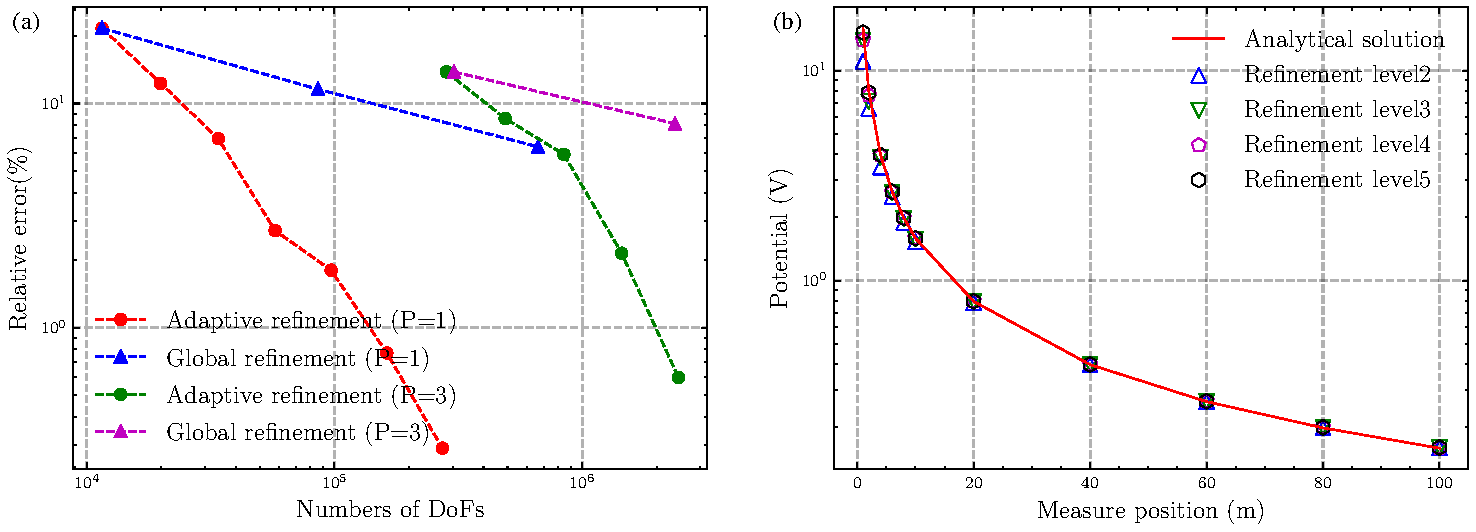
\includegraphics[width=1\linewidth]{fig/halfspace_relative_err.pdf}
  \caption{When the basis functions are first-order and third-order, (a) the curves of the relative error using different grid refinement strategies. The relative error is calculated by averaging the relative error of the numerical solution for all receivers compared to the analytical solution. (b) The curves of potential at measuring points with different refinement levels. }
  \label{fig:halfspace_relative_err}
\end{figure}
% \begin{figure}\ContinuedFloat \centering \subfloat[Third-order basis
%   function]{\includegraphics[width=1\linewidth]{fig/Potentialvalue3.pdf}\label{fig:sub3}}\\
%   \subfloat[Fourth-order basis
%   function]{\includegraphics[width=1\linewidth]{fig/Potentialvalue4.pdf}\label{fig:sub4}}
%   \caption{When the basis functions are third-order (c) and fourth-order (d),
%   the curves of the relative error using different grid refinement strategies
%   and the curves of potential at measuring points with different refinement
%   levels.} \label{fig:Potentialvalue34} \end{figure}
\begin{figure}
  \centering
  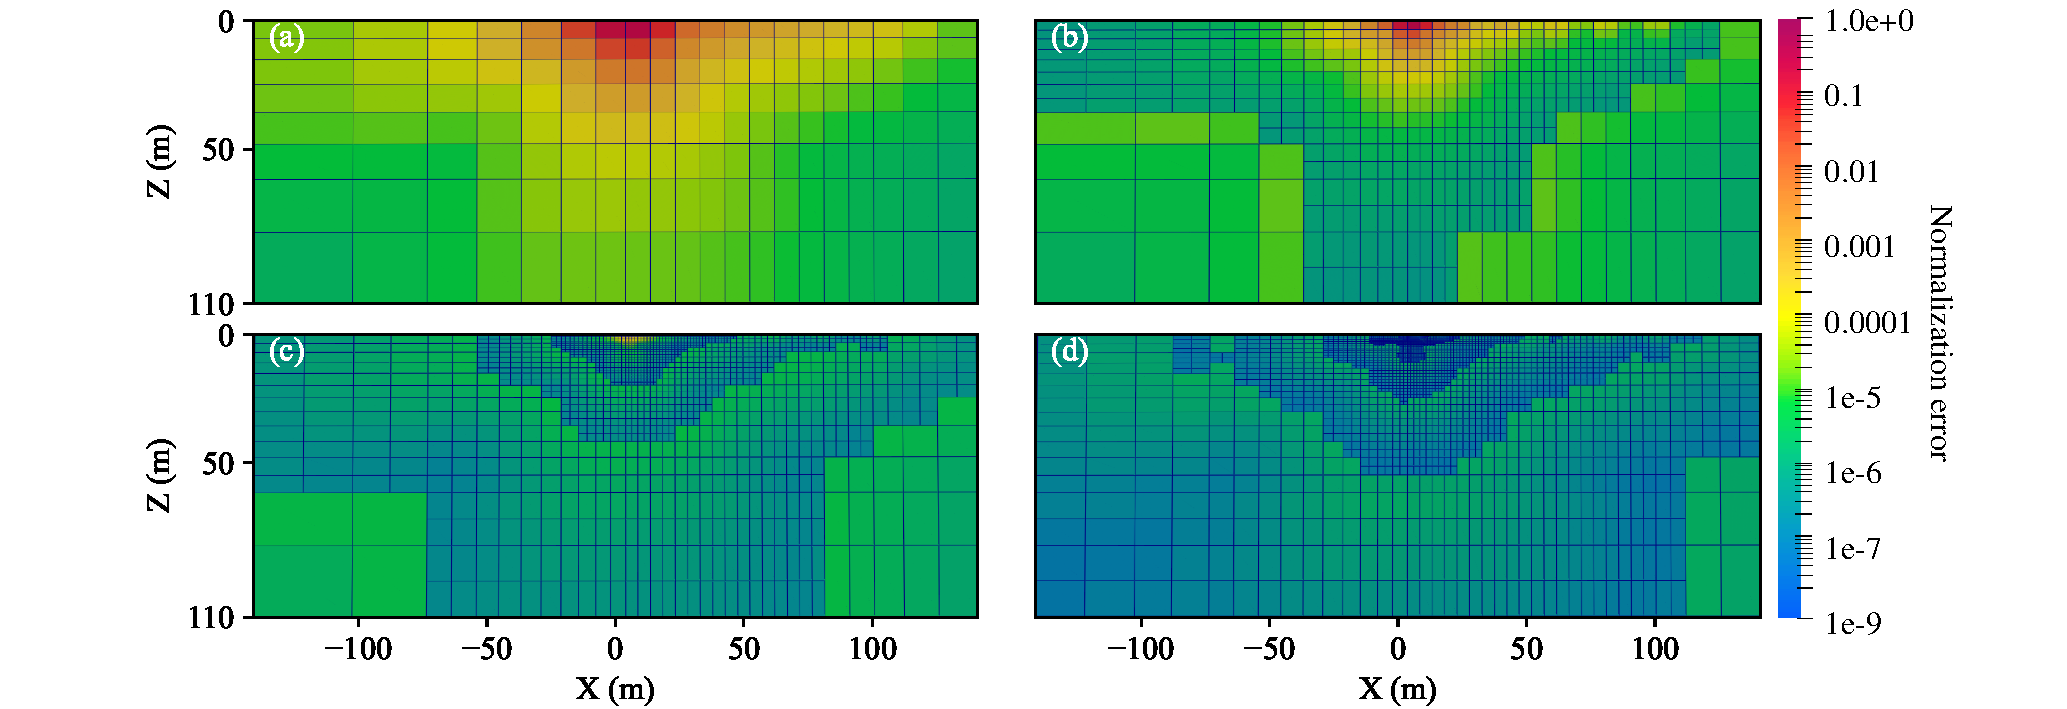
\includegraphics[width=1.0\textwidth]{fig/halfsapce_adaptive_effect.pdf}
  \caption{Illustrative diagram of the $xoz$ cross-section mesh of (a) initial model, (b) the first refined grids, (c) the third refined grids, and (d) the fifth refined grids. After normalizing the error, the posterior error within the target area is demonstrated.}
  \label{fig:halfsapce_adaptive_effect}
\end{figure}

% For further exploration into the adaptive algorithm's convergence, we
% conducted numerical simulations on the mentioned model employing higher-order
% basis functions. Figures 5(b)(c)(d) display the relative error curves obtained
% from the two refinement strategies employing high-order basis functions, along
% with the curves representing the numerical and analytical solutions. It's
% evident that the adaptive algorithm continues to exhibit lower relative errors
% and an accelerated precision increase rate when utilizing high-order basis
% functions, emphasizing the robustness of the adaptive algorithm. Moreover,
% with an increase in the basis function's order, the adaptive algorithm attains
% higher-precision solutions requiring fewer refinements. These findings
% emphasize the adaptive algorithm's superiority over global refinement in
% enhancing solution accuracy and optimizing memory usage.

\subsection{Comparison between GMG and AMG}
To compare the performance between GMG and AMG, we selected three scenarios. Fig
\ref{fig:two_scenarios} displays two of the three scenarios, presenting side-view
diagrams, which include background resistivity and abnormal bodies information.
\begin{figure}
  \centering
  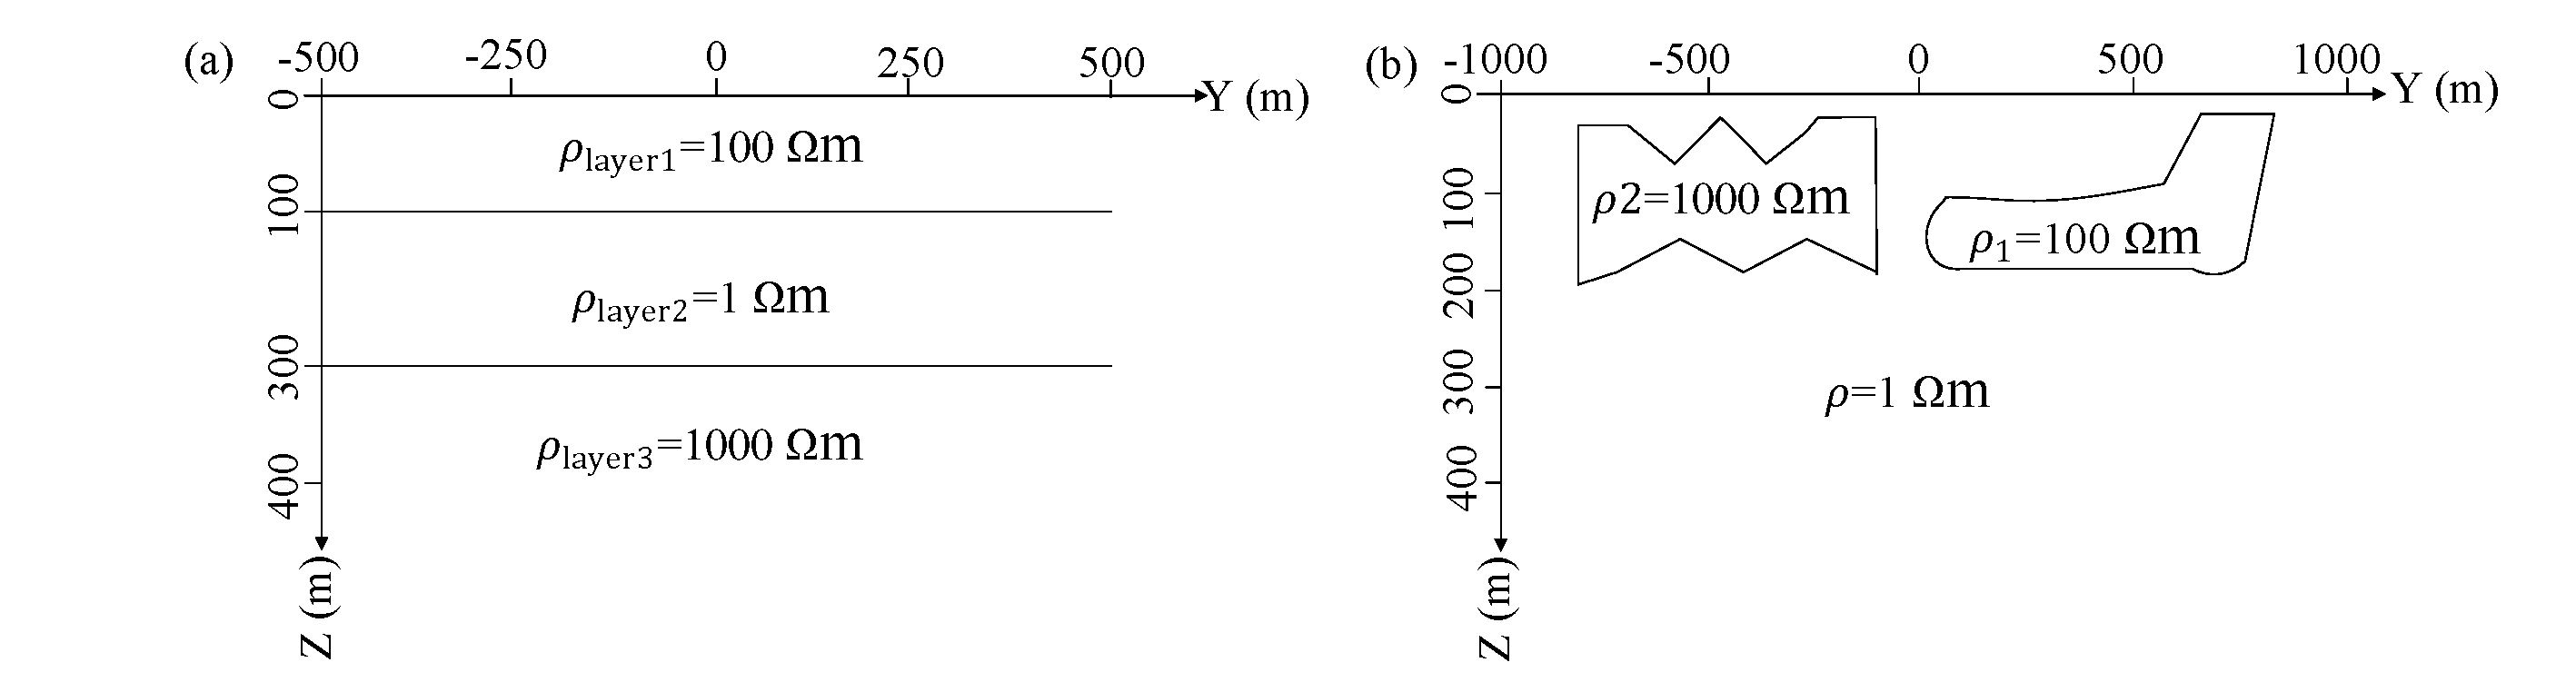
\includegraphics[width=1\textwidth]{fig/two_scenarios.pdf}
  \caption{The cross-sectional schematic diagram of the models used to test the performance of GMG and AMG includes conductivity information. Scenario 1 (a) and scenario 2 (b). For illustrative purposes, the figure is not drawn to scale.}
  \label{fig:two_scenarios}
\end{figure}
\begin{figure}
  \centering
  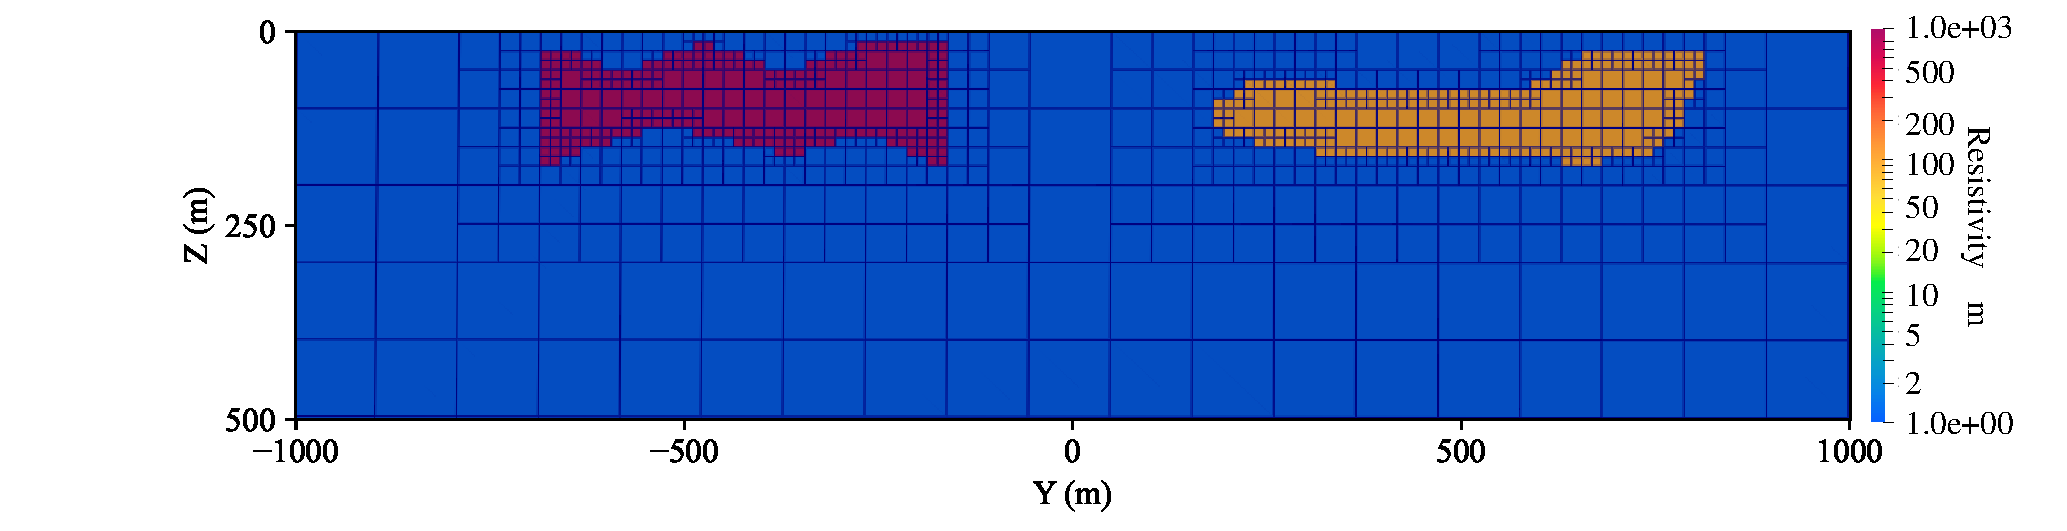
\includegraphics[width=1\textwidth]{fig/complex_model.pdf}
  \caption{The cross-sectional diagram depicting the $YoZ$ plane of the octree-modeled structure for model 3. The coordinate of the source electrode is (0\,m,0\,m,0\,m).}
  \label{fig:complex_model}
\end{figure}
\begin{figure}
  \centering
  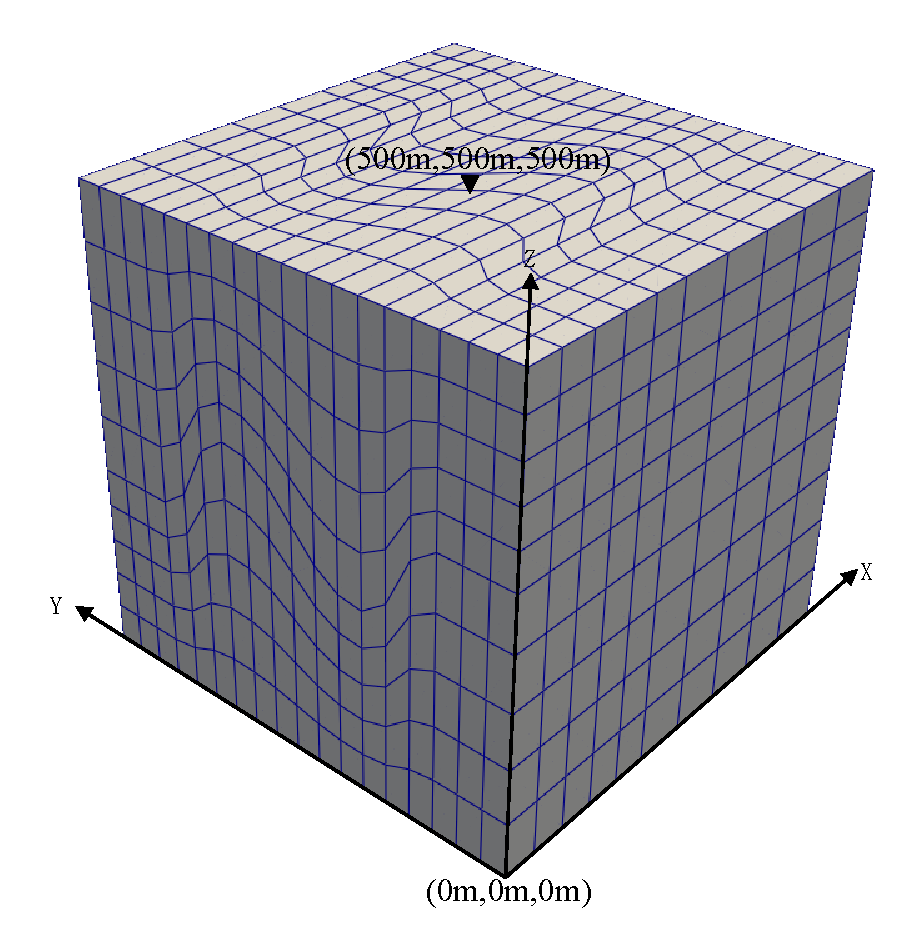
\includegraphics[width=0.6\textwidth]{fig/unstructured_model.pdf}
  \caption{Visualization of scenario 2, illustrating the mesh partition of the Kershaw grid. The anisotropic parameters for the mesh are $\varepsilon_y=0.8$ and $\varepsilon_z=0.8$.}
  \label{fig:unstructured_model}
\end{figure}

Scenario 1: a three-dimensional layered model as shown in Figure
\ref{fig:two_scenarios}(a), with layer-wise resistivity of 100 $\Omega m$, 1
$\Omega m$, and 1000 $\Omega m$. The initial number of elements for this model
is 64. The model has a depth of 400 meters and a width of 1000 meters. We
supplied power at the position (0\,m, 0\,m, 0\,m) with a current of 1A.

Scenario 2: a three-dimensional model measuring 13\,km × 13\,km × 6\,km is
considered. Within the range of the $y-axis$ from -1000\,m to +1000\,m and the
range of the $x-axis$ from -300\,m to +300\,m, there are two irregular abnormal
bodies. The background resistivity is 1 $\Omega m$, while the abnormal bodies
have resistivity of 1000 $\Omega m$ and 100 $\Omega m$, respectively. Figure
\ref{fig:two_scenarios}(b) illustrates a $YoZ$ section diagram of the model at
x=0\,m. We employed an octree grid to discretize this computational domain. As
shown in Fig. \ref{fig:complex_model}, the octree grid accurately represents the
complex shape of the abnormal bodies. For our experimental setup, we arrange the
transmitter and receiver devices following the Schlumberger sounding
configuration. The transmitting electrodes were uniformly positioned within the
span from (0\,m, -2000\,m, 0\,m) to (0\,m, 2000\,m, 0\,m) with a 50-meter
spacing. Similarly, observation points were uniformly distributed from (0\,m,
-1000\,m, 0\,m) to (0\,m, 1000\,m, 0\,m), also maintaining a 50-meter spacing.
The receiver devices are positioned along the $y-axis$ at a distance of 2.5
meters on both side of the observation points.

Scenario 3: we considered a Kershaw grid, where the spatial dimensions measure
1\,km × 1\,km × 1\,km, featuring a background resistivity of 100 $\Omega m$. The
power supply is located at (500\,m, 500\,m, 500\,m), and the model has 2299
elements. As shown in Fig. \ref{fig:unstructured_model}, our grid is obtained by
deforming a uniform grid, deforming the cells along the deformation curve
\citep{Kershaw1981}. The characteristics of Kershaw grid are defined by two
anisotropic parameters, $\varepsilon_y$ and $\varepsilon_z$. Similar to the
approach outlined in \citep{Camier2023}, the anisotropic parameters used for our
model: $\varepsilon_y=0.8$ and $\varepsilon_z=0.8$.

We first employed GMG and AMG to separately calculate the responses of the
scenario 1. Due to the absence of additional refinement in the cells within
scenario 1, GMG divides the grid into only one level. This causes GMG to switch
directly to a coarse-grid solver, making the iteration count meaningless at this
stage.
\begin{table}
    \centering
    \caption{The solving time and number of iterations of AMG and GMG method. We
      apply global refinement to the model of scenario 1. During the initial
      computation, NA is used to replace the GMG's solving time and number of
      iterations.}
    \begin{tabular}{lcccc}
    \toprule
    \multirow{2}{*}{Degrees of Freedom} & \multicolumn{2}{c}{Solving time (s)} &
    \multicolumn{2}{c}{Number of iterations} \\ \cmidrule(lr){2-3}
    \cmidrule(lr){4-5} & AMG & GMG & AMG & GMG \\ \midrule 64 & 0.00109 & NA & 4
    & NA \\
    343 & 0.00141 & 0.00569 & 5 & 4 \\
    2197 & 0.0137 & 0.00695 & 5 & 4 \\
    15625 & 0.082 & 0.0219 & 5 & 5 \\
    117649 & 0.935 & 0.167 & 6 & 5 \\
    912673 & 10.4 & 1.33 & 7 & 5 \\
    7189057 & 84.6 & 10.7 & 7 & 5 \\ \bottomrule
    \end{tabular}
    \label{table:first}
\end{table}

Table \ref{table:first} presents the solving time and iteration counts of the CG
solver for scenario 1 using AMG and GMG. The results indicate that as the
degrees of freedom increase, GMG consistently demonstrates higher solving
efficiency and fewer iteration counts compared to AMG. For the degrees of
freedom amount to 117649, the solving time for GMG is 0.167 seconds, roughly
one-sixth of AMG's time. This advantage becomes notably more pronounced as the
degrees of freedom increase. Moreover, the iteration count for GMG stabilizes at
5, fewer iterations than AMG requires to meet the preset tolerance. This
indicates that, compared to AMG, the CG solver combined with GMG completes each
iteration in less time.
\begin{figure}
  \centering
  % \subfloat{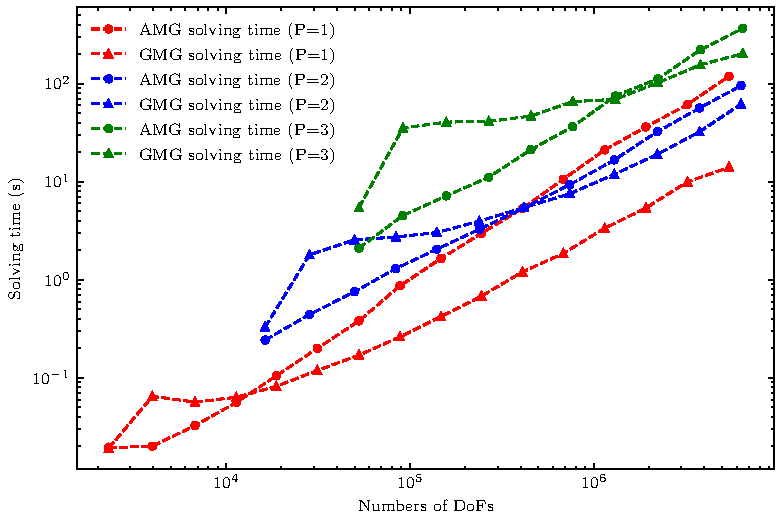
\includegraphics[width=1\linewidth]{fig/results_unstructured_model.pdf}\label{fig:sub2}}
  % \subfloat[]{\includegraphics[width=0.3\linewidth]{fig/AGcompare2bl.pdf}\label{fig:sub3}}
  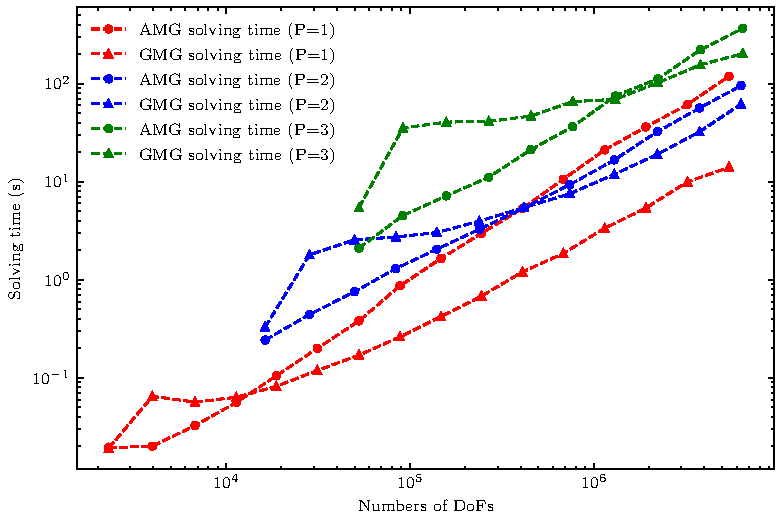
\includegraphics[width=0.8\linewidth]{fig/results_unstructured_model.pdf}
  \caption{The solving time curves for the model of scenario 2. The curves show the solving time obtained by applying GMG and AMG under different orders of basis functions. }
  \label{fig:results_unstructured_model}
\end{figure}

Subsequently, we conducted numerical simulations for scenario 2 to investigate
the capability of GMG in providing accurate solutions in complex scenarios. The
cells at the edges of the abnormal body exhibit a higher refinement level in
scenario 2. In geometric multigrid methods, highly refined cells may cross
different resistivity regions after local smoothing, potentially impacting the
iterative solving process. To mitigate this, at grid level l, we modify the
resistivity information of the current grid by employing the average value of
the subdomain resistivity. To visually illustrate the electrical potential
distribution of the model, we utilize Schlumberger Vertical Electrical Sounding
(VES) \citep{Constable1984,Gance2014} technique to calculate apparent
resistivity and generate a pseudo-section.
\begin{figure}
  \centering
  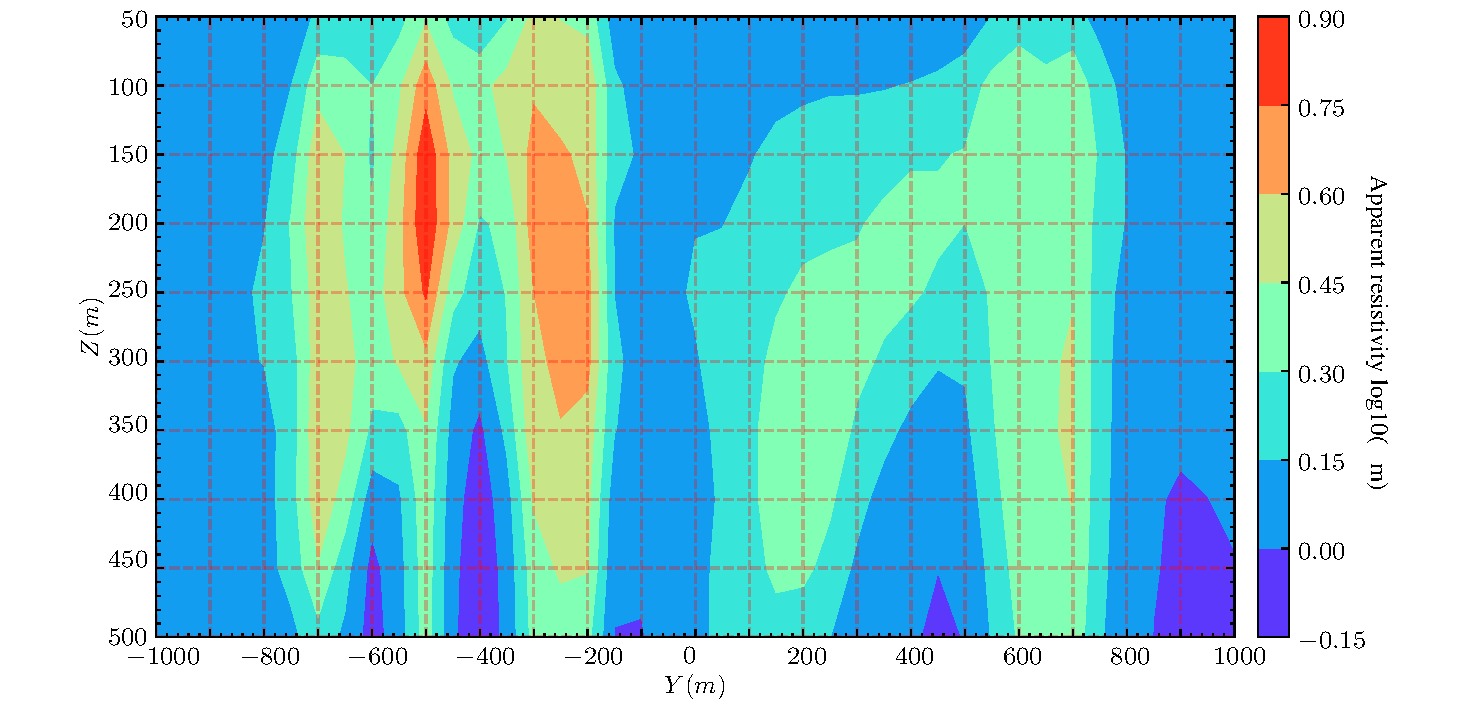
\includegraphics[width=1\textwidth]{fig/pseudo-section.pdf}
  \caption{The pseudo-section plot obtained using Schlumberger sounding accurately depicts different resistivity zones in relative terms. Regarding data accuracy, the apparent resistivity data in the plot is based on a grid refined through three times adaptive refinement.}
  \label{fig:pseudo-section}
\end{figure}
Fig. \ref{fig:pseudo-section} shows a pseudo-section derived from a
cross-sectional view at X=0m which extends in the Y direction from -1000\,m to
1000\,m and in the Z direction from 0\,m to 1000\,m. The apparent resistivity
correctly represents the relative resistivity relationship between two abnormal
bodies and the background. The pseudo-section displays two distinct
high-resistivity abnormal region, whose positions and outlines correspond to the
abnormal bodies in scenario 3. It is noteworthy that the pseudo-section plot
displays clear boundaries between the abnormal bodies and the background.

Finally, we utilized higher-order basis functions to conduct numerical
simulations for scenario 3, investigating the performance of GMG under
unstructured model. In Fig. \ref{fig:results_unstructured_model}, we show the solution time
curves for AMG and GMG under different basis functions. At first, due to the
lower refinement levels of the grid, the GMG was unable to split the grid into
sufficient levels to accelerate the solving process. Therefore, during the
initial few adaptive refinements, the GMG's solving time exceeded that of AMG.
However, after 3 to 5 adaptive refinements, the solving time of the GMG became
lower than that of AMG, demonstrating higher performance. It is noteworthy that
because GMG initially divides the model into only one level, the computation
time for the initial model is similar for both AMG and GMG at this stage. These
results demonstrate that GMG is more suitable for solving large-scale matrices
when dealing with unstructured grids.


\subsection{Various stretch factor}
In finite element analysis, an increase in the stretch factor leads to an
increase in the condition number of the linear system of equations. According to
the results in \citep{Ern2006}, higher condition numbers often result in
decreased solution accuracy or may lead to instability in the solver.

In this section, we employed grids with various stretch factors to assess the
stability of GMG. Initially, we constructed a half-space model as the initial
model, where the computational domain of the initial model was $\Omega =
(-150\,m, 150\,m)^3$. The initial model comprised 216 cells, each measuring 50
meters in length, width, and height. When the grid is split into only one grid
level, GMG will directly solve on the coarse grid, leading to an incorrect
iteration count. To address this issue, cells within the region of
$(-100\,m,100\,m)^3$ are generated by refining once the cells of size 100.
Subsequently, we adjusted the grid's stretch factor by introducing five padding
cells along the positive and negative directions of the X, Y, and $Z-axes$ of
the initial grid. These padding cells increased proportionally in size. We
placed the transmitter at coordinates (0\,m, 0\,m, 0\,m).

We conducted simulations on models with different stretch factors. Table
\ref{table:stretch} provides the computational time of numerical simulations
employing GMG and AMG methods, along with the iteration count of the CG solver.
The table shows  that with an increase in the models' stretch factor, the
solving time of GMG consistently remains lower than that of AMG. Moreover, GMG
maintains a stable iteration count at 3, while AMG exhibits significant
deterioration in performance as the condition number increases. These results
indicate that GMG can maintain excellent computational stability while achieving
higher solution efficiency in scenarios with large condition numbers.

% When the computational domain is fixed, this capability enables us to create
% initial models with larger stretch factors while ensuring accuracy in the
% target area. For instance, when considering a stretch factor of 2.4 in the
% scenario depicted in the table \ref{table:stretch}, the computational domain
% is $\Omega = (-1950, 1950)^3$, and the initial degree of freedom is 4096.
% However, when modeling with a uniform grid and maintaining precision in the
% central region of the grid, the initial degree of freedom for the established
% model amounts to 474552. As a result, there is a significant reduction in the
% initial degrees of freedom count, thereby boosting the efficiency of
% subsequent numerical simulations.
\begin{table}
    \centering
    \caption{The numerical simulation time using GMG and AMG methods along with
      the iteration count of the CG solver for models with varying scaling
      factors.}
    \begin{tabular}{lcccc}
    \toprule
    \multirow{2}{*}{Stretch factor} & \multicolumn{2}{c}{Solving time (s)} &
    \multicolumn{2}{c}{Number of iterations} \\ \cmidrule(lr){2-3}
    \cmidrule(lr){4-5} & AMG & GMG & AMG & GMG \\ \midrule 1.2 & 0.0282 & 0.0228
    & 5 & 4 \\
    1.4 & 0.0399 & 0.0275 & 6 & 4 \\
    1.6 & 0.0596 & 0.0318 & 10 & 3 \\
    1.8 & 0.0892 & 0.0408 & 15 & 3 \\
    2.0 & 0.109 & 0.0553 & 21 & 3 \\
    2.2 & 0.129 & 0.0755 & 27 & 3 \\
    2.4 & 0.142 & 0.0867 & 35 & 2 \\
    2.6 & 0.189 & 0.126 & 44 & 3 \\  \bottomrule
    \end{tabular}
    \label{table:stretch}
\end{table}


\subsection{Parallel scalability}

In this section, we applied the message passing interface (MPI) protocol to
evaluate the parallel efficiency of GMG. Scalability, as discussed by
\citep{Buntinas2008}, stands as a critical metric for assessing the MPI parallel
algorithm's performance. It represents the system's capability to maintain or
enhance its performance when additional computing resources like CPUs, memory,
and network bandwidth are introduced. The efficacy of parallel algorithms is
assessed using the acceleration ratio, computed via the following formula:
\begin{equation}
   {S}_{p}= \frac{{T}_{1}}{{T}_{p}},
\end{equation}
where p denotes the number of processes, ${T}_{1}$ represents the time required
to solve the problem using a single CPU, and ${T}_{p}$ denotes the time required
to solve the problem using p processes simultaneously.

In this experiment, a half-space model is utilized and the initial computational domain spans $3615 \times 3615 \times 2077$ $m^3$, featuring 6615 elements. The MPI parallel program was simulated using 1, 2, 4, 8, 16, 32, and 64 processes. For grids with different degrees of freedom, Fig. \ref{fig:results_parallel1} and \ref{fig:results_parallel2} show the speedup and the solving time required using different numbers of processes.

\begin{figure}
  \centering
  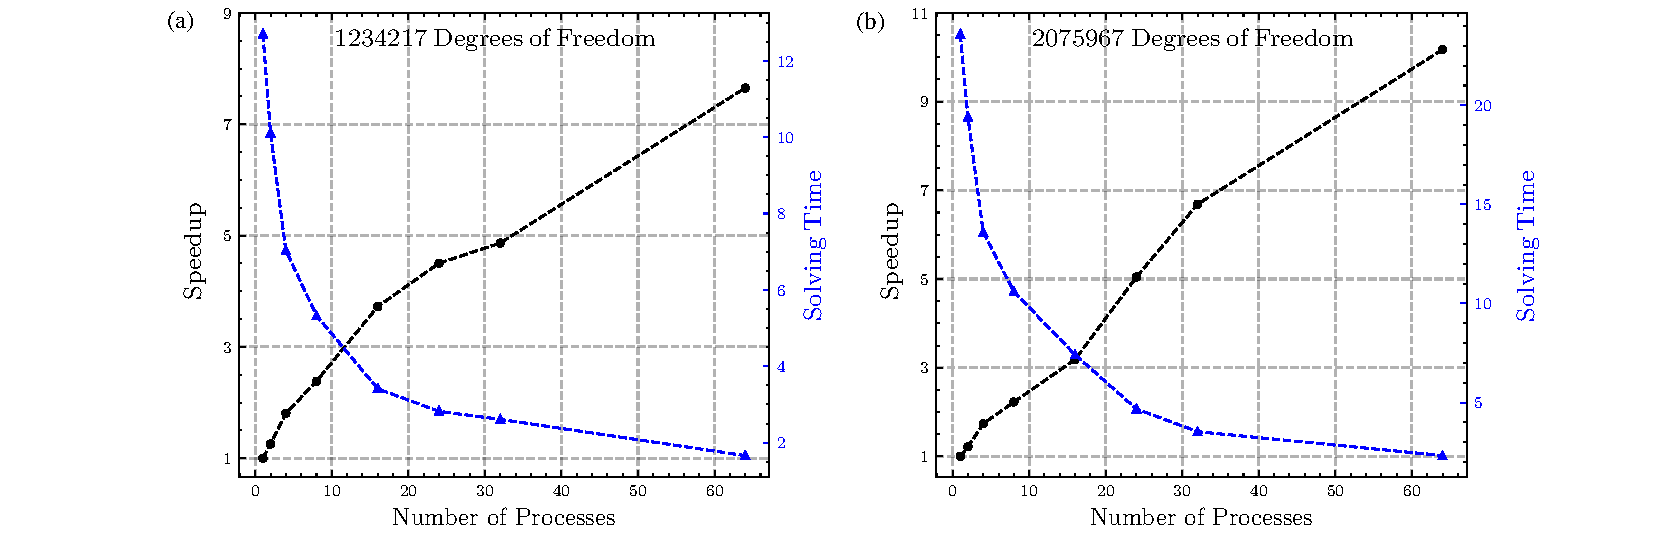
\includegraphics[width=1\textwidth]{fig/results_parallel1.pdf}
  \caption{The curves of speedup and solving time under different MPI processes when the degrees of freedom are 1234517 and 2075967 respectively.}
  \label{fig:results_parallel1}
\end{figure}
\begin{figure}
  \centering
  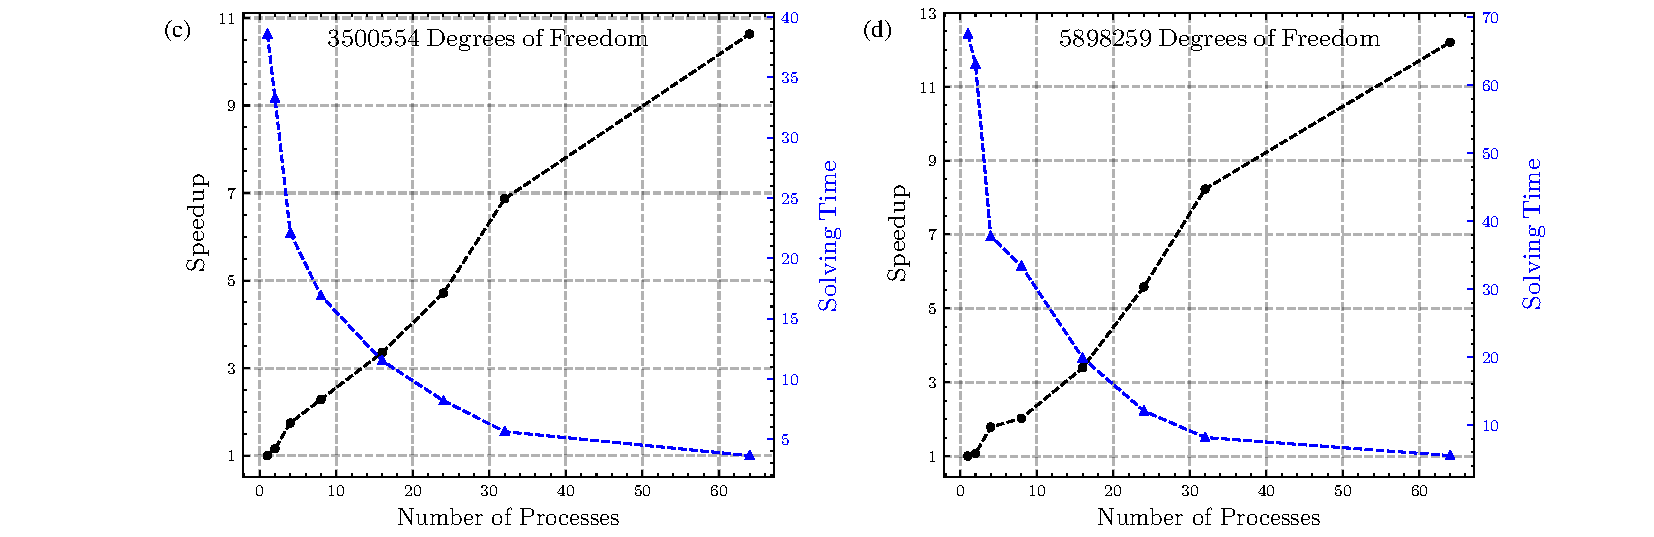
\includegraphics[width=1\textwidth]{fig/results_parallel2.pdf}
  \caption{The curves of speedup and solving time under different MPI processes when the degrees of freedom are 3500554 and 5898259 respectively.}
  \label{fig:results_parallel2}
\end{figure}


As shown in Fig. \ref{fig:results_parallel1}, with lower degrees of freedom, an increase in
the number of processes can not result in a rise in speedup. This is because,
with smaller computational scales, the data exchange between different processes
constitutes a larger portion of the total time, resulting in lower speedup
ratios. When considering Fig. \ref{fig:results_parallel1} and Fig. \ref{fig:results_parallel2}, the
parallel speedup of GMG improves with increasing computational scale. This trend
suggests GMG's suitability for large-scale parallel computing, showcasing
commendable scalability. However, the changes of slope within these figures
indicate that with higher degrees of freedom, augmenting the number of processes
might not yield substantial performance enhancements. In fact, an increase in
number of processes might heighten communication overhead, directly impacting
overall system performance. Therefore, achieving optimal parallel efficiency
requires considering factors such as degrees of freedom, the number of
processes, and communication overhead in tandem.



\bibliographystyle{gji}
\bibliography{reference}

\end{document}
